\documentclass[letterpaper]{article}
\usepackage[utf8]{inputenc}
\usepackage[parfill]{parskip}    % Activate to begin paragraphs with an empty line rather than an indent
\usepackage{graphicx}
\usepackage{amssymb}
\usepackage{amsmath}
\usepackage{amsthm}

\usepackage{afterpage}

\usepackage{algorithm}
\usepackage{algpseudocode}

\usepackage{verse}

\newtheorem{theorem}{Theorem}[section]
\newtheorem{corollary}{Corollary}[theorem]
\newtheorem{lemma}[theorem]{Lemma}

\theoremstyle{remark}
\newtheorem*{remark}{Remark}

\usepackage{epstopdf}
\usepackage{circuitikz}
\usepackage[separate-uncertainty = true,multi-part-units=single]{siunitx}
\usepackage{booktabs}
\usepackage{enumitem}
\usepackage[toc,page]{appendix}
\usepackage{color}
\usepackage{pgfplots}
\usepackage{pgfplotstable}
\usepackage{caption}
\usepackage{subcaption}
\usepackage{url}
\usepackage{multirow}
\usepackage{makecell}
\usepackage[round]{natbib}   % omit 'round' option if you prefer square brackets
\usepackage{titling}
\usepackage{siunitx}

\usepackage{setspace}
% \doublespacing
\usepackage{float}


\pgfplotsset{compat=1.14}

%  Special math symbols
%       floor, ceiling, angled brackets
%-----------------------------------------------------------------------
\newcommand{\floor}[1]{\left\lfloor #1\right\rfloor}
\newcommand{\ceil}[1]{\left\lceil #1\right\rceil}
\newcommand{\etal}{\textit{et al.}}
\newcommand{\RE}{\mathbb{R}}        % real space
\newcommand{\ZZ}{\mathbb{Z}}        % integers
\newcommand{\NN}{\mathbb{N}}        % natural numbers
\newcommand{\eps}{{\varepsilon}}    % prettier epsilon
%-----------------------------------------------------------------------
%  Tighter lists
%-----------------------------------------------------------------------
\newenvironment{itemize*}% Tighter itemized list
  {\begin{itemize}%
    \setlength{\itemsep}{-0.5ex}%
    \setlength{\parsep}{0pt}}%
  {\end{itemize}}
\newenvironment{description*}% Tighter description list
  {\begin{description}%
    \setlength{\itemsep}{-0.5ex}%
    \setlength{\parsep}{0pt}}%
  {\end{description}}
\newenvironment{enumerate*}% Tighter enumerated list
  {\begin{enumerate}%
    \setlength{\itemsep}{-0.5ex}%
    \setlength{\parsep}{0pt}}%
  {\end{enumerate}}
%-----------------------------------------------------------------------
% Typing shortcuts
%-----------------------------------------------------------------------
\newcommand{\X}{\mathbb{X}}
\newcommand{\SG}{\mathbf{S}}
\newcommand{\GE}{\mathcal{G}}
\newcommand{\ST}{\,:\,}
\renewcommand{\tilde}[1]{\widetilde{#1}}
\newcommand{\diam}{\mathrm{diam}}
\newcommand{\sq}{\square}
\newcommand{\half}[1]{\frac{#1}{2}}
\newcommand{\inv}[1]{\frac{1}{#1}}
\newcommand{\alg}{\textsf{SplitReduce}}
\newcommand{\sz}[1]{\sigma_{#1}}
\newcommand{\LL}{\mathcal{L}}
\newcommand{\softOmega}{\widetilde{\Omega}} 
\newcommand{\softO}{\widetilde{O}}
\newcommand{\OO}{O^*}  %or \widetilde{O}?

\newcommand{\norm}[1]{\left\lVert#1\right\rVert}

\newcommand{\dx}{\mathrm{d}x}
\newcommand{\dy}{\mathrm{d}y}
\newcommand{\dz}{\mathrm{d}z}
\newcommand{\dt}{\mathrm{d}t}
\newcommand{\du}{\mathrm{d}u}
\newcommand{\dtheta}{\mathrm{d}\theta}
\newcommand{\dq}{\mathrm{d}q}
\newcommand{\diff}{\mathrm{d}}
\newcommand{\dV}{\mathrm{d}V}
\newcommand{\dL}{\mathrm{d}L}
\newcommand{\dA}{\mathrm{d}A}
\newcommand{\dH}{\mathrm{d}H}
\newcommand{\df}{\mathrm{d}f}
\newcommand{\dg}{\mathrm{d}g}
\newcommand{\dr}{\mathrm{d}r}
\newcommand{\dw}{\mathrm{d}w}
\newcommand{\dv}{\mathrm{d}v}

\newcommand*\len[1]{\overline{#1}}

\newcommand{\dd}{Decadent Dwight cookies }
\newcommand{\hh}{Heavenly Hearst cookies }

\newcommand\note[1]{\marginpar{\textcolor{red}{#1}}}
\newcommand*{\tageq}{\refstepcounter{equation}\tag{\theequation}}

\newcommand*{\equals}{=}

\usepackage{fancyhdr}

\pgfplotscreateplotcyclelist{grayscale}{
    thick,white!10!black,mark=x,mark options=solid, dashed\\%
    thick,white!20!black,mark=o,mark options=solid\\%
}

\newcommand{\mat}[1]{\ensuremath{\begin{bmatrix}#1\end{bmatrix}}}
\newcommand{\eqn}[1]{\begin{alignat*}{2}#1\end{alignat*}}
\newcommand{\p}[2]{\frac{\partial #1}{\partial #2}}
\newcommand*{\thus}{&\implies\quad&}

\newcommand{\answer}[1]{\framebox{$\displaystyle #1 $}}

 
\pagestyle{fancy}
\fancyhf{}
\rhead{Rahul Arya}
\lhead{EE 16B}
\cfoot{\thepage}

\title{Lecture 3 - Notes}
\author{Rahul Arya}
\date{January 2019}
\begin{document}

\maketitle

\section{Overview}
In the first lecture, we viewed transistors as ``magic" components, with the position of a switch between two terminals controlled by the voltage at a third terminal. In the second, we saw that transistors in reality have an internal resistance and capacitance, and studied their effects on the behavior of digital circuits. Now, we will investigate the physical construction of transistors and other semiconductor-based components.

\section{Atomic Models}
First, though, we will consider various models of the atom. The classical model of an atom is the \emph{planetary model}, with negatively charged, light particles known as \emph{electrons} orbiting around a heavy, positively charged central body known as the \emph{nucleus}, made up of positively charged \emph{protons}. Both protons and electrons have the same magnitude of charge, which we will denote as $\pm e$.

However, this model fails to explain several physical observations - in particular, atomic absorption and emission lines. These lines can be observed by exciting a gas formed of a single type of atom, and measuring the frequency of light emitted. We observe that this emitted light is composed of light of only a few different frequencies - for instance, excited hydrogen gas only emits visible light of the frequencies \SI{656}{\nano\meter}, \SI{486}{\nano\meter}, \SI{434}{\nano\meter},  \SI{410}{\nano\meter}, \SI{397}{\nano\meter}, and \SI{364}{\nano\meter}. Similarly, when monochromatic light at (or very near) these frequencies is shone into hydrogen gas, it is absorbed to a far greater extent than light of other frequencies \footnote{IIRC, the reason that light of other frequencies is also absorbed is due, in part, to the frequency shift of incoming light from the perspective of moving atoms within the gas}.

These observations become more interesting when we consider the photon model of light. Here, light is viewed to be composed of small packets of energy known as \emph{photons}. The energy of each packet is dependent solely on its frequency - specifically, $E = hf$, where $E$ is the energy of the photon, $h$ is Planck's constant, and $f$ is the frequency. Thus, we find that atoms emit and absorb photons only with particular frequencies, a phenomenon that is entirely unexplained by the planetary model.

The Bohr model of the atom resolves this issue very elegantly. Its key assumption is that of the quantization of electron \emph{angular momentum} - that is, the angular momentum of the electrons orbiting the nucleus cannot take on arbitrary values, but rather must be a multiple of the constant $\hslash = \frac{h}{2\pi}$. It can be shown that this, in turn, quantizes the energy levels of these electrons, forcing them into discrete \emph{orbitals} around the nucleus, with the orbitals increasing in energy the further they are from the nucleus. When an atom is excited, an electron moves from one energy level $E_2$ to another of higher energy $E_1$. When this atom then returns to a ground state, this electron drops back to its original energy level, emitting a photon with energy $\Delta E = E_1 - E_2$, and frequency $f = \frac{E_1 - E_2}{h}$. Clearly, the discrete nature of these energy levels constrains $\Delta E$ to a discrete set of frequencies, which form the emission spectrum of the atom.

One property of these atomic orbitals is known as the \emph{Pauli exclusion principle}. For our purposes, we may interpret this property as stating that each energy level can only hold a finite number of electrons. Silicon, which is a semiconductor, has at ground state $14$ electrons distributed across the shells $1s^2$, $2s^2$, $2p^6$, $3s^2$, and $3p^2$, as shown:
\begin{center}
    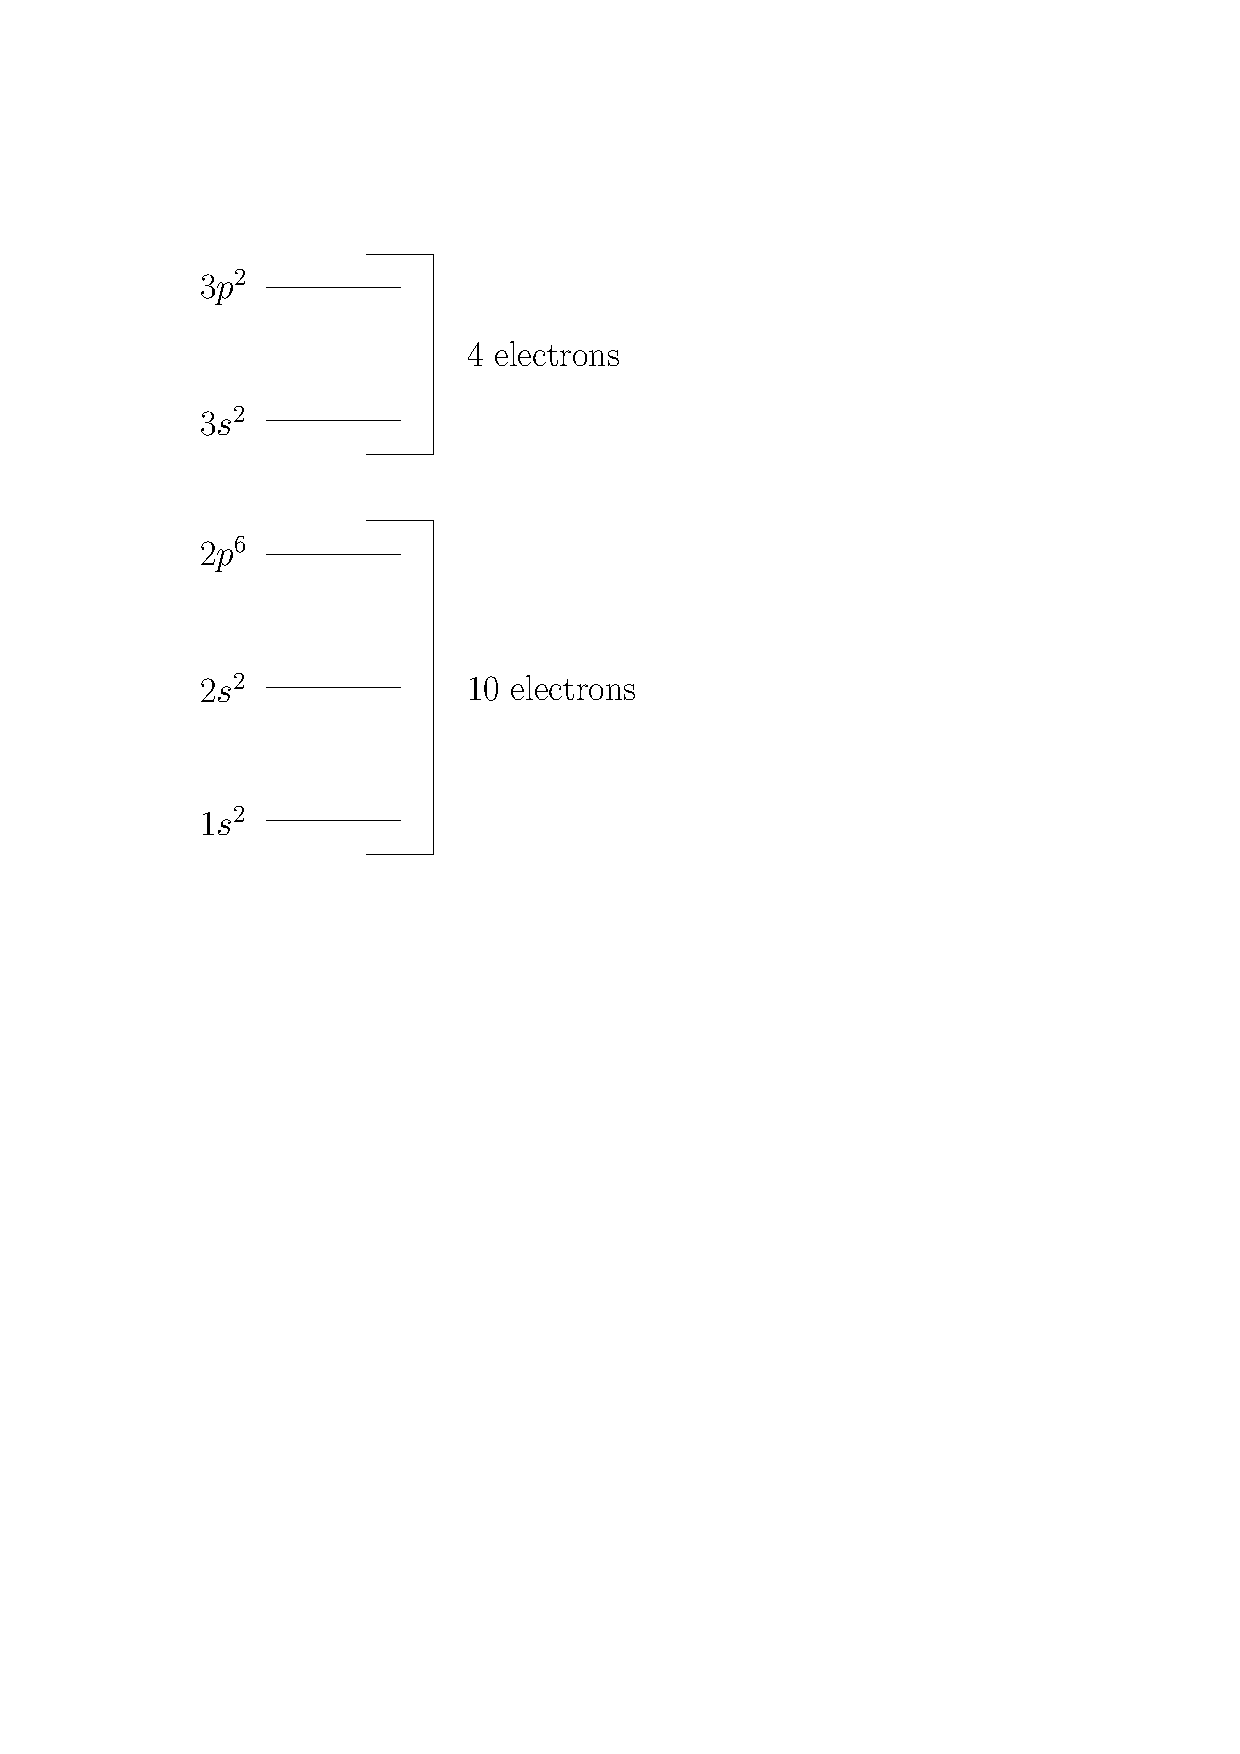
\includegraphics[scale=0.7]{si_shells.pdf}
\end{center}
(note that the superscript denotes the number of electrons contained in each energy level).

Note that atoms tend towards lower energy states, which is why energy levels higher than shown are unoccupied. However, the electrons cannot all occupy the lowest energy state, and so form this configuration, which minimizes their total energy while obeying the Pauli exclusion principle. In addition, it is important to note that the $4$ electrons at the highest energy levels (known as valence electrons) can move around more freely within a silicon crystal, whereas the lower $10$ electrons remain firmly bound to their atom's nucleus.

\section{A Silicon Crystal}

In a silicon crystal of $N$ electrons (where $N$ is very large), additionally (unlike in a single atom), we can view the composition of these discrete energy levels from all the different silicon atoms in the crystal to form \emph{energy bands} as the number of atoms rises, as shown:
\begin{center}
    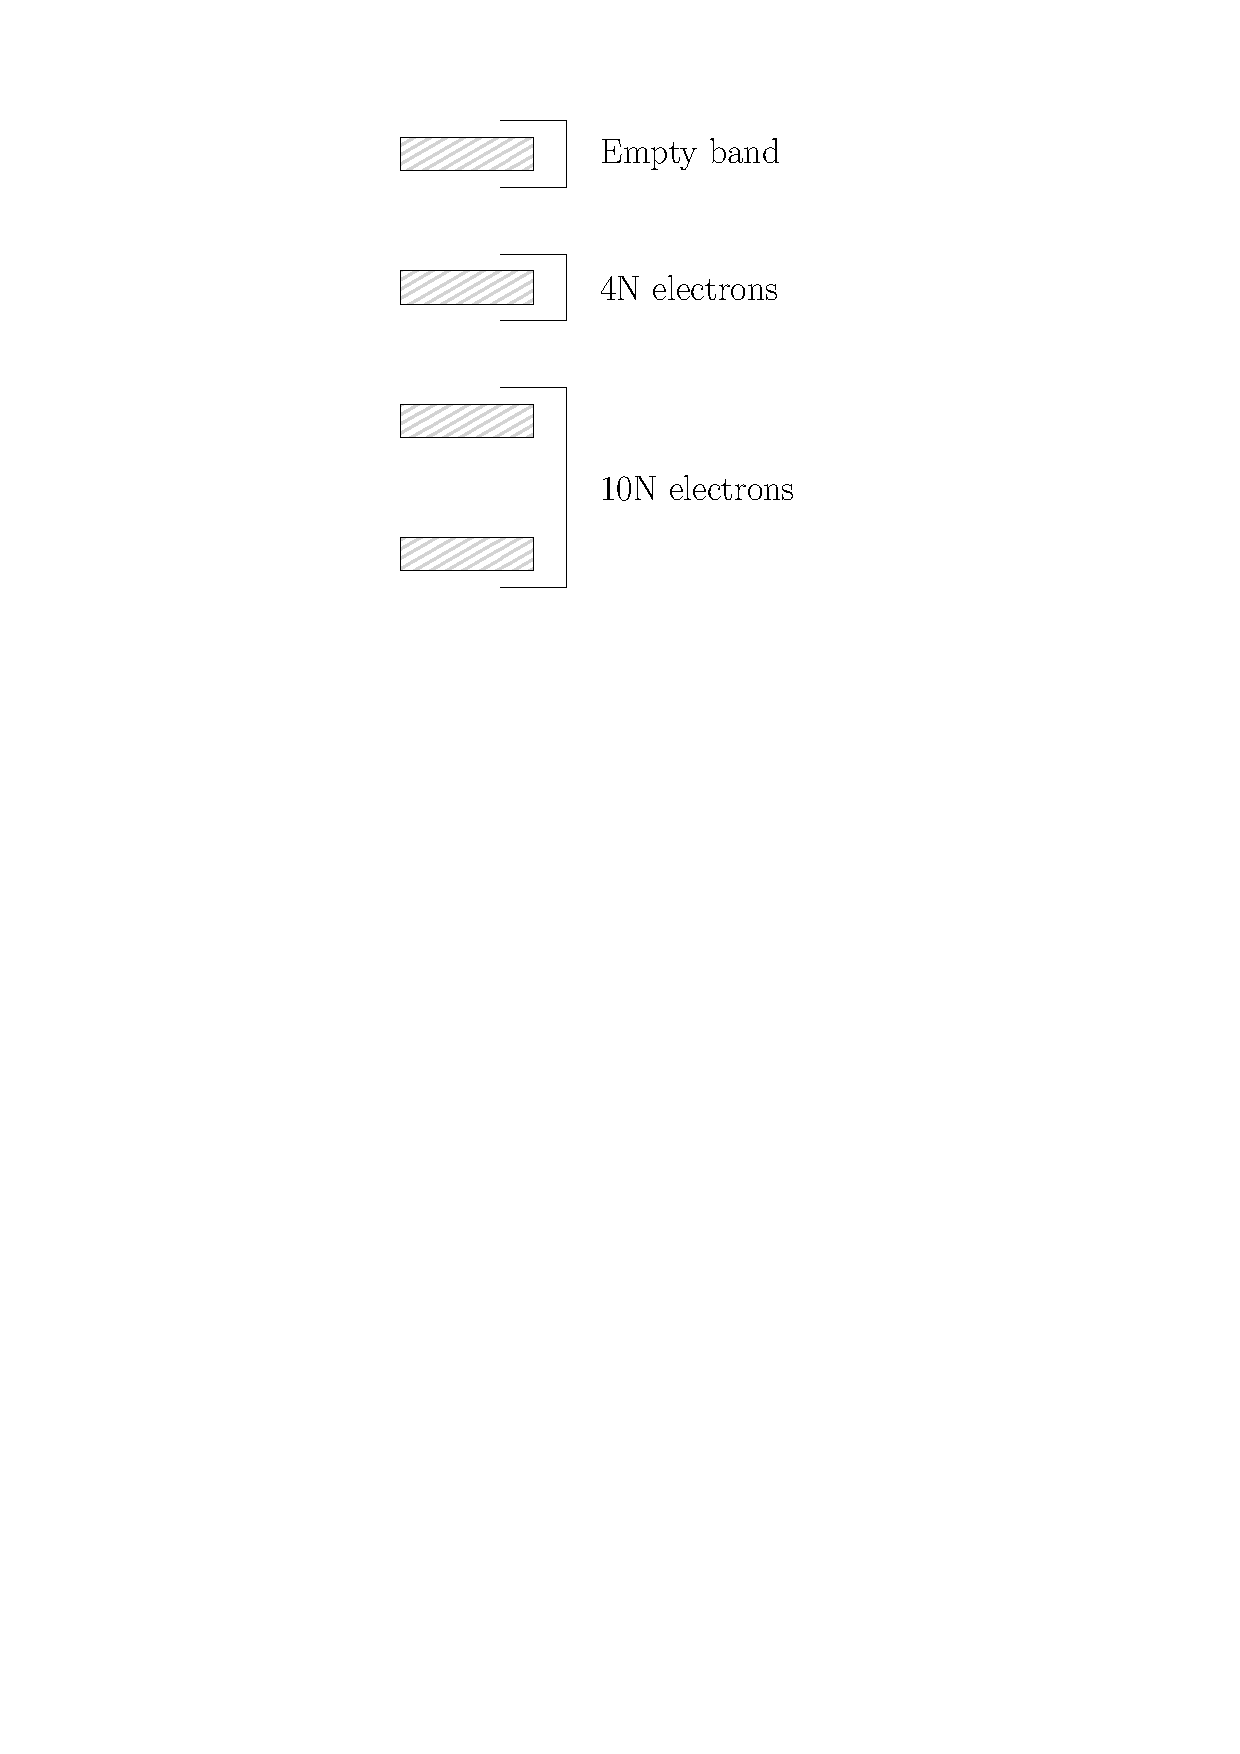
\includegraphics[scale=0.7]{si_crystal.pdf}
\end{center}

In particular, note that all the valence electrons lie in the highest nonempty energy band - known as the \emph{valence band} - which is fully occupied. Since electrons in lower energy bands don't move between atoms, we are no longer interested in them. Also observe that we have drawn the energy band just above the valence band - this band is known as the \emph{conduction band}, and will shortly be of interest. While electrons may occupy what is effectively a continuous interval of energy levels within energy bands, it is impossible for electrons to remain between these energy bands.

First, we will redraw our picture to focus on just these two bands:
\begin{center}
    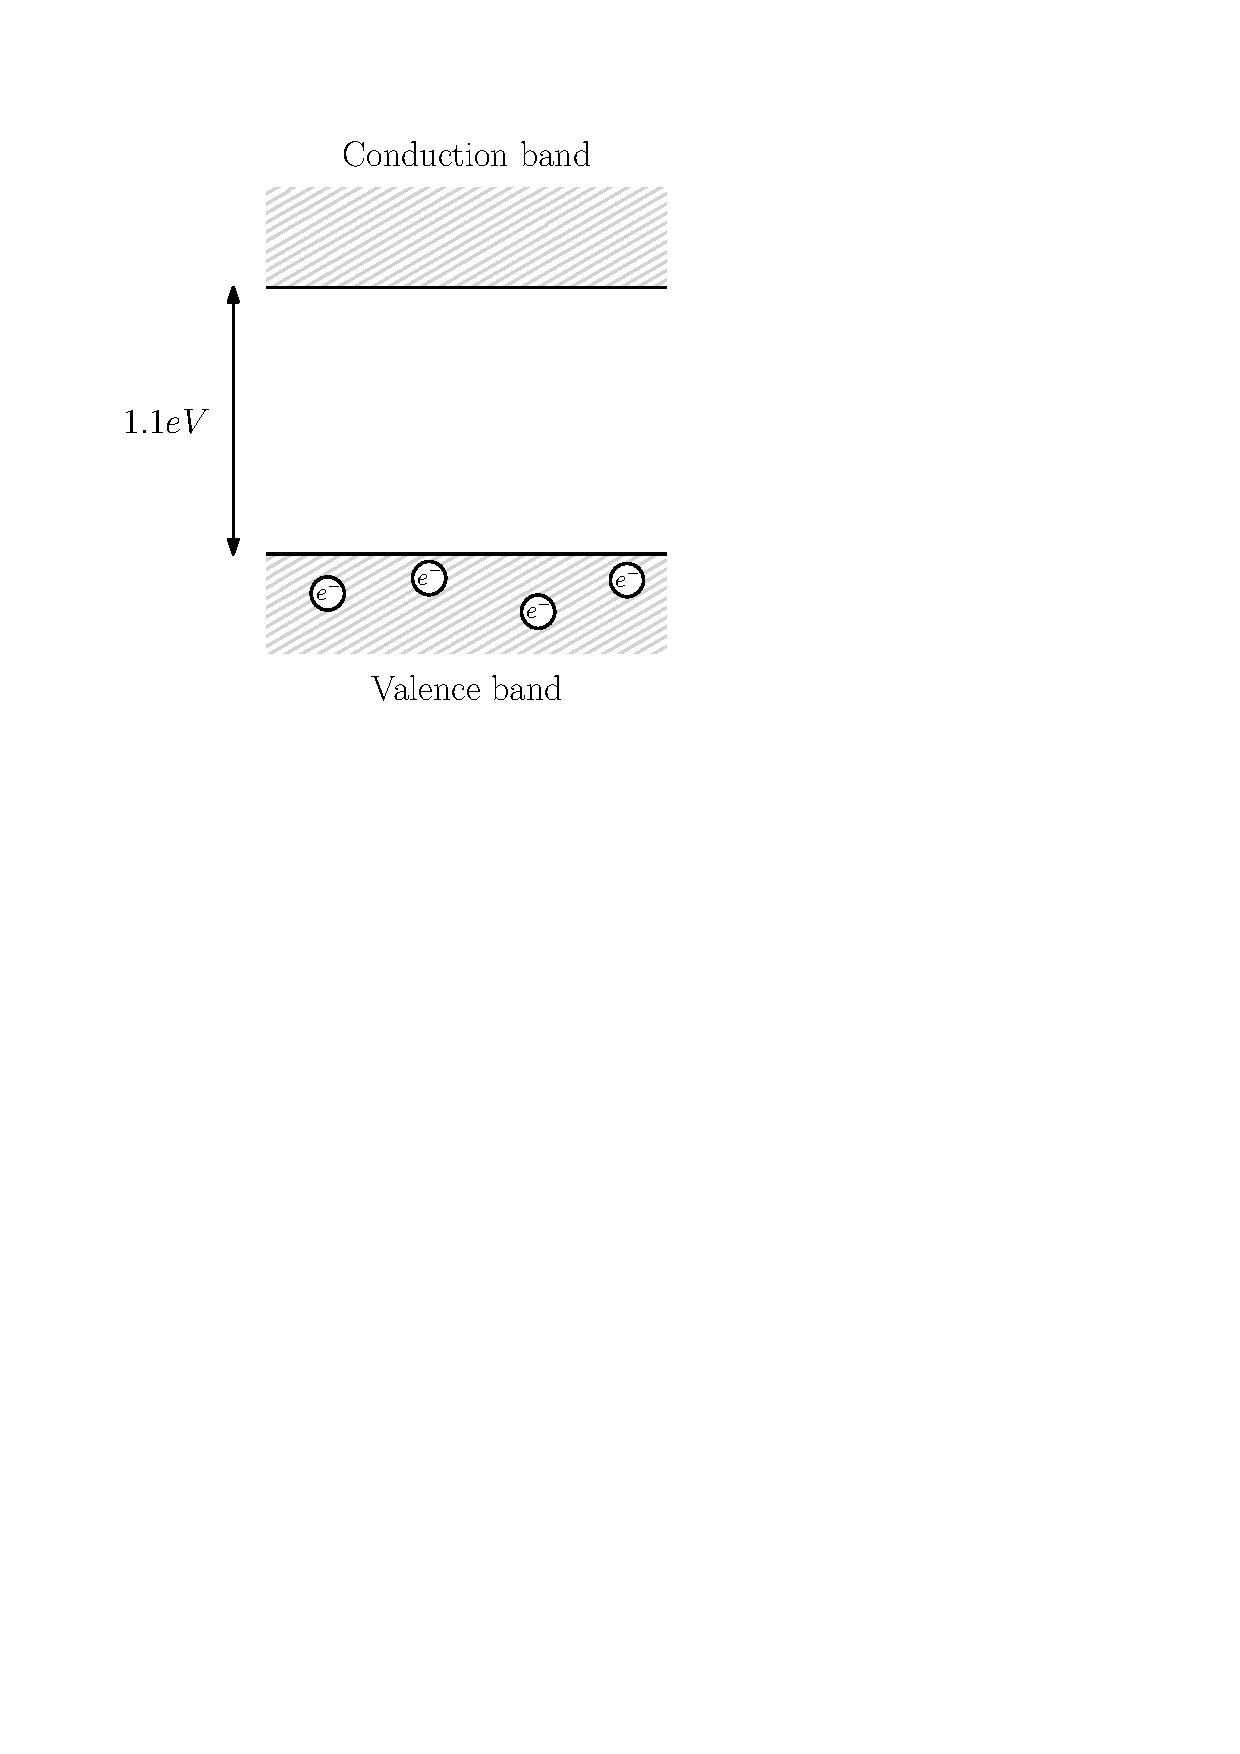
\includegraphics[scale=0.7]{si_band_gap.pdf}
\end{center}

On the left, we have labeled the energy gap between these two energy bands, known as the \emph{band gap}. This represents the minimum energy required for an electron to jump from the valence band to the conduction band or, equivalently, the energy released when an electron drops from the conduction band to the valence band. Note that we label higher energy bands as vertically above lower energy bands, but this is done purely for visual clarity - in reality, electrons of differing energy levels all live around the nucleus of their atom, with electrons further from the nucleus occupying higher energy levels, on average.

Now, we will apply a voltage across a silicon crystal, and observe what happens to the electrons:
\begin{center}
    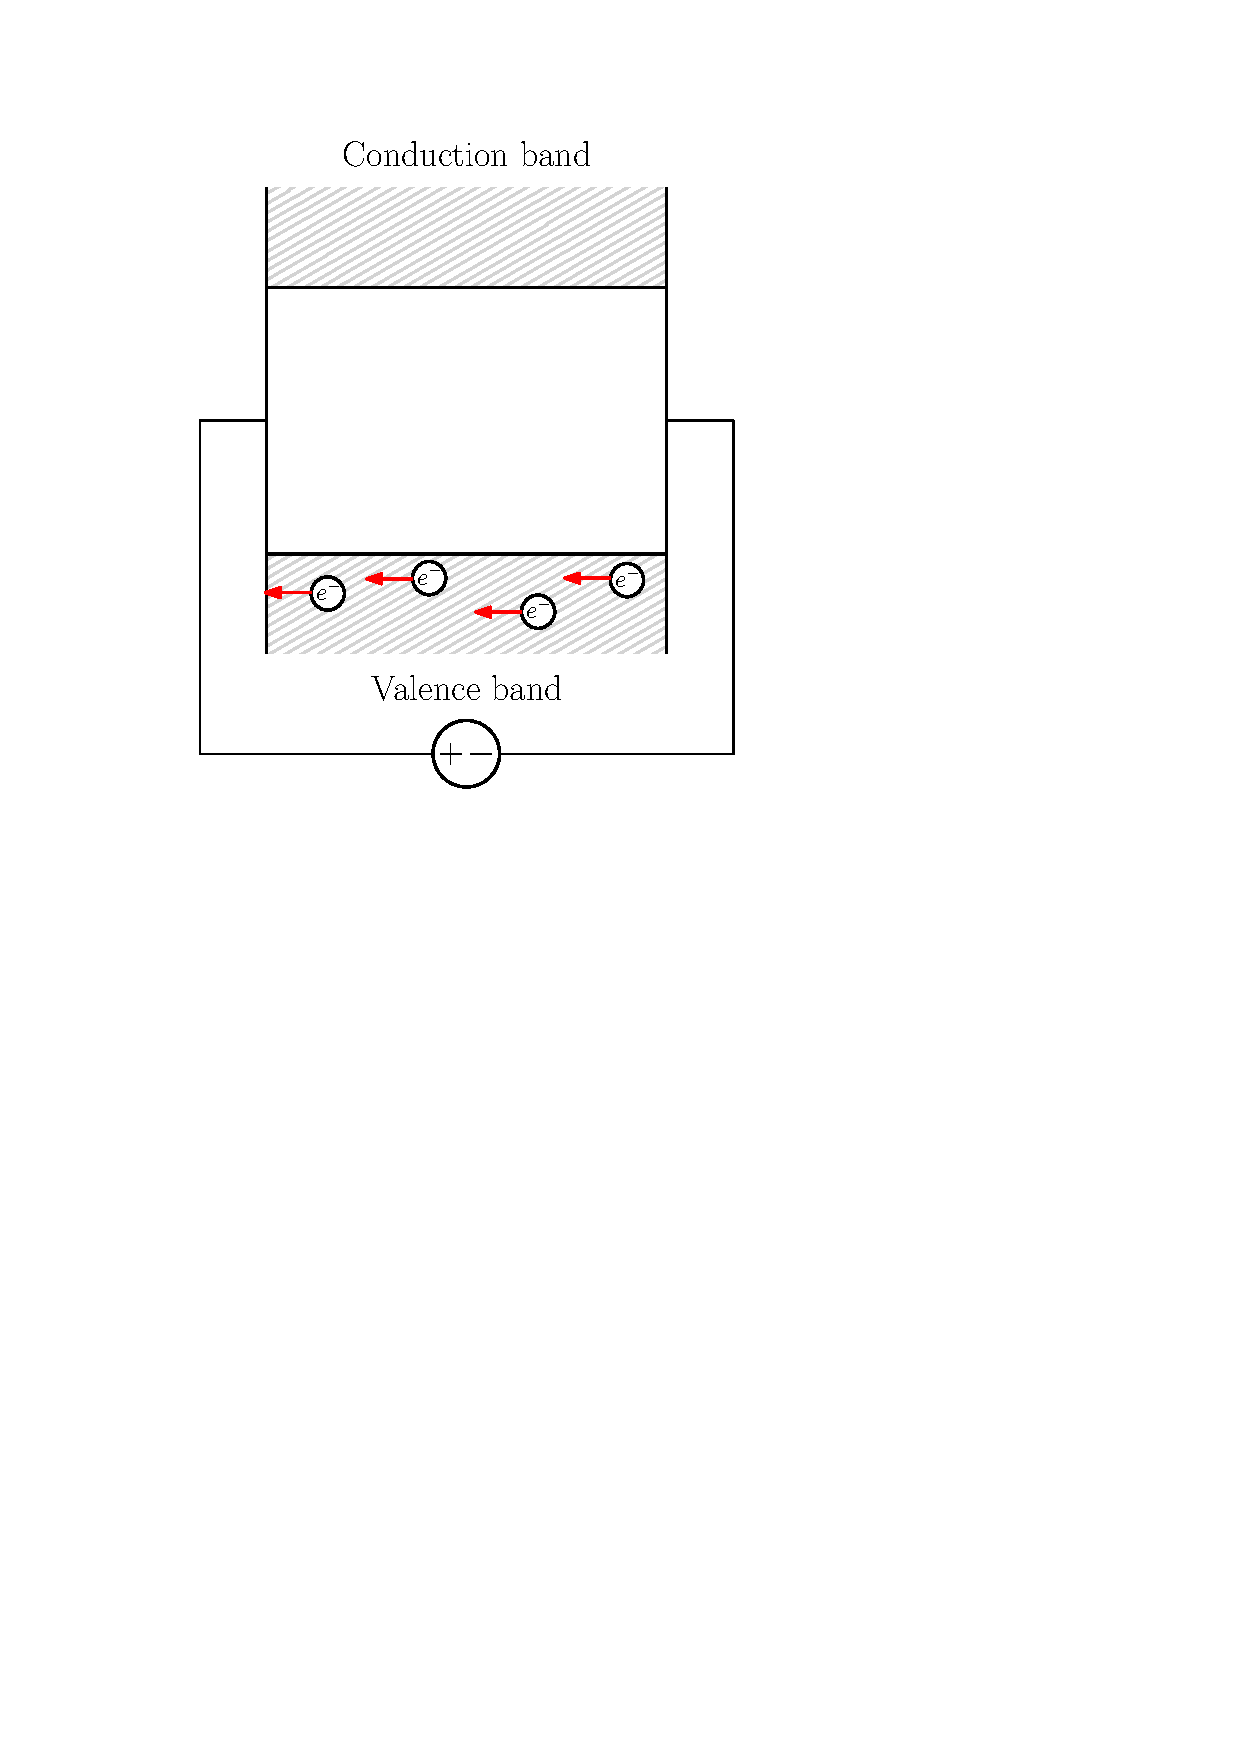
\includegraphics[scale=0.7]{si_voltage_band.pdf}
\end{center}

The voltage source produces an electric field within the crystal directed to the right. Thus, the electrons (being negatively charged) experience a force to the left. Despite this force, as the valence band has no empty space, the electrons are unable to move. Thus, when all the electrons are in the valence band, the silicon crystal acts as an insulator.

\section{Effects of Heat and Light}
However, due to thermal excitation, some of the electrons in the valence band may ``jump" to the conduction band, leaving a \emph{hole} in the valence band. Alternatively, if the crystal is exposed to light, then electrons may again be excited and jump to a higher energy band. If this is the case, then the excited electron will lie in an almost entirely empty energy band, meaning that it can freely move in response to the electric field, meaning that an current is induced, known as the \emph{electron current}. Less obviously, the hole left in the valence band will appear to move rightwards with the electric field, inducing a further positive current to the right (known as the \emph{hole current}). This mechanism is summarized in the following figure:
\begin{center}
    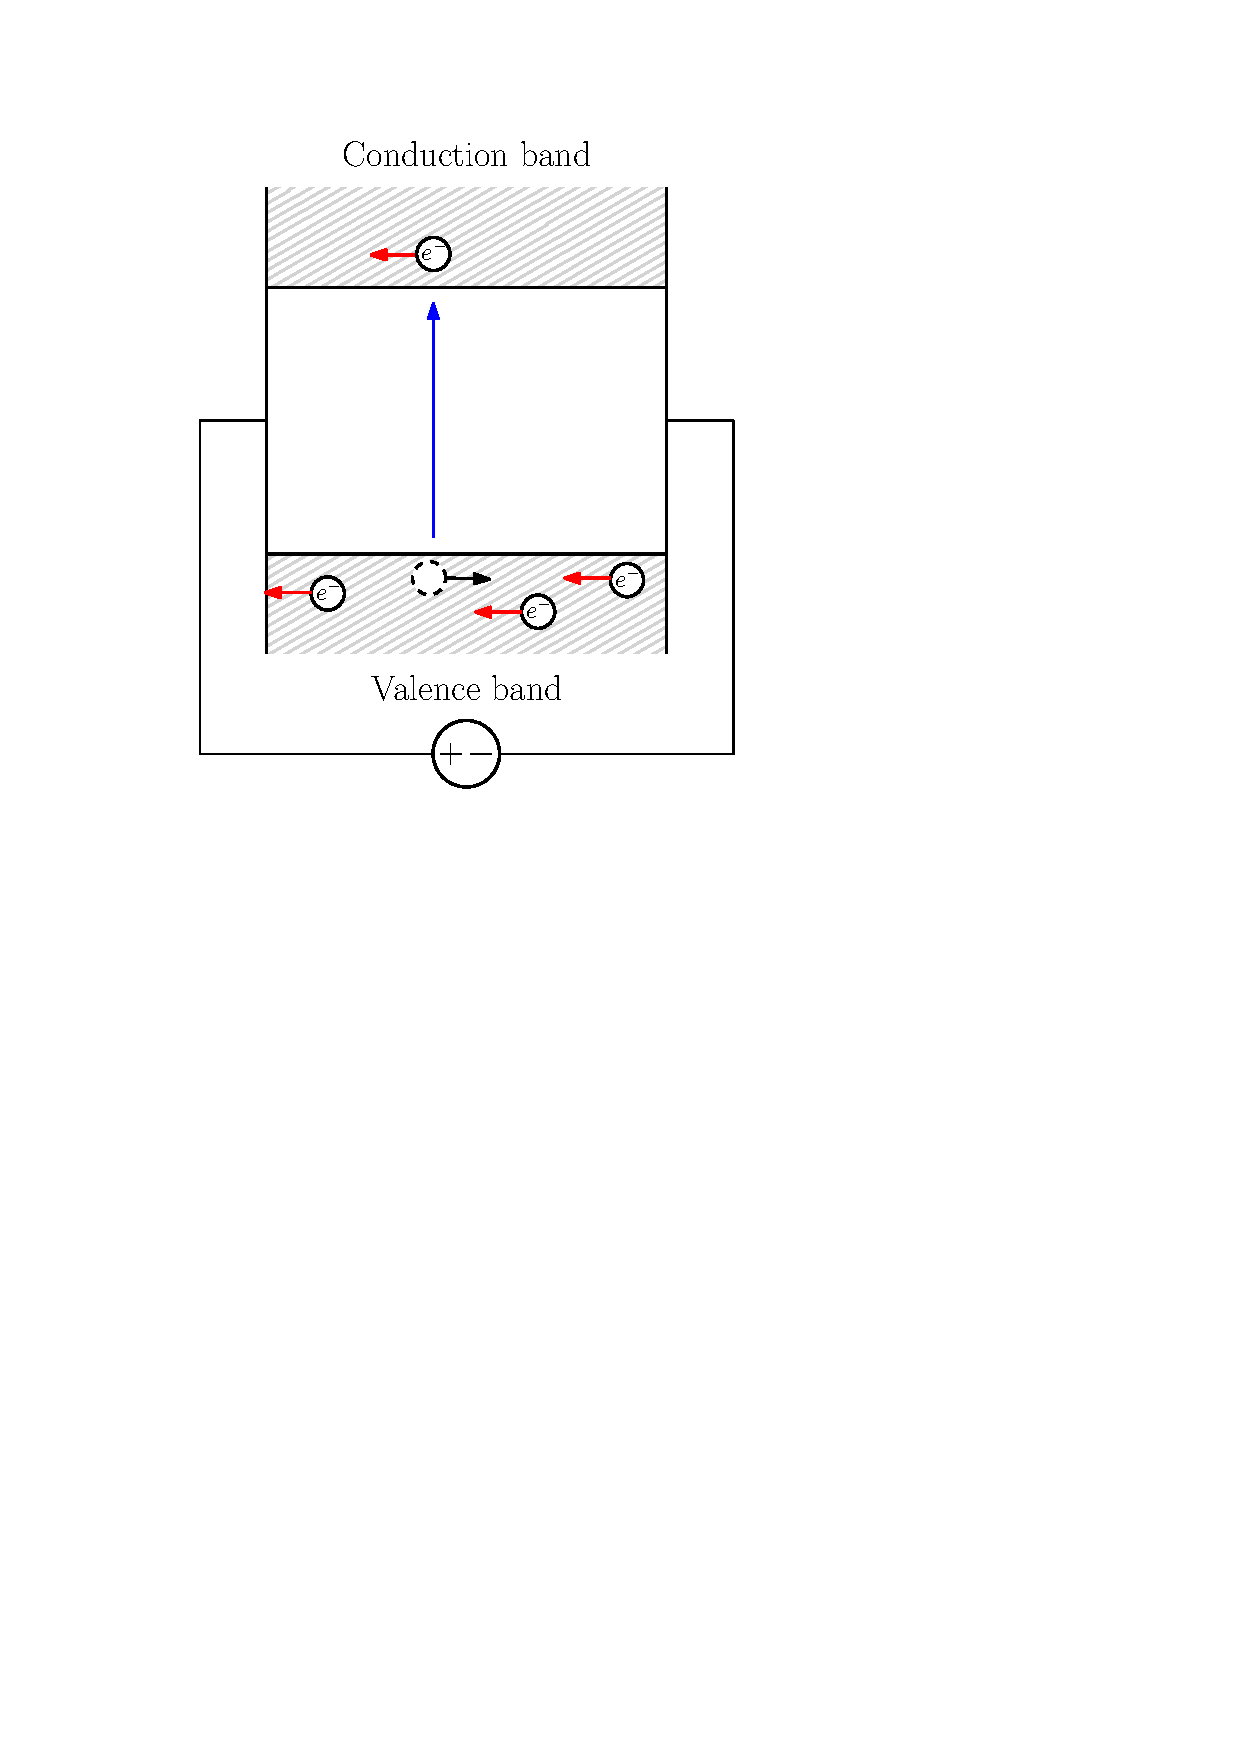
\includegraphics[scale=0.7]{si_excited_electrons.pdf}
\end{center}
Of course, the hole is not a physical object, and so does not experience any forces directly. Rather, the surrounding electrons, driven by the electric field, move to fill the hole, ``pushing" the hole to the right. This mechanism is analogous to the motion of bubbles rising in a drink - while they may appear to move upwards, it is really the surrounding drink's motion downwards that creates the bubbles' apparent motion.

As mentioned previously, photons can excite electrons, pushing them into the conduction band. Over a very short duration of time, these electrons will lose energy in the conduction band, falling continuously to the lower bound of the conduction band. As their energy continues to dissipate, they will drop abruptly to the valence band, emitting a photon of a very precise frequency (that corresponding to the band gap), even when the initial photon had energy greater than the band gap, as shown below:
\begin{center}
    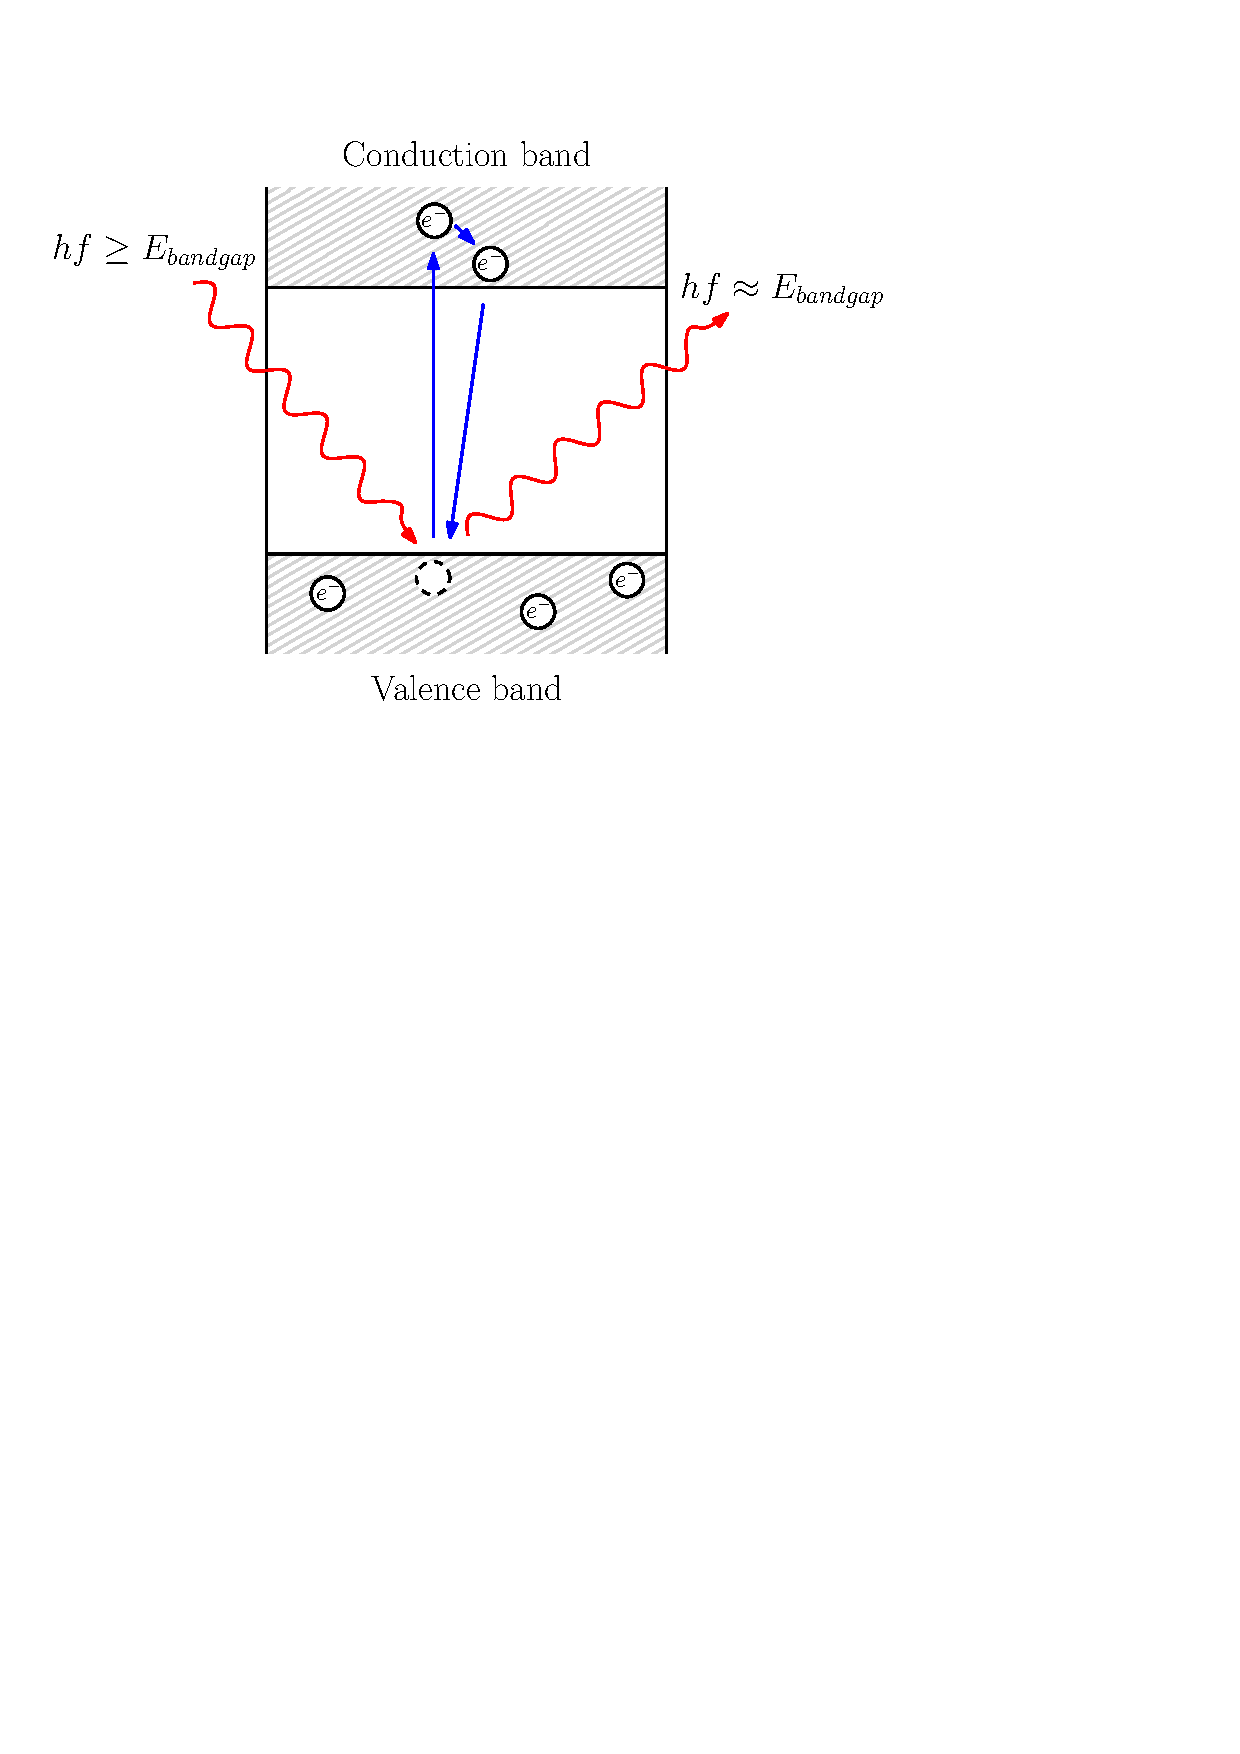
\includegraphics[scale=0.7]{si_photon_absorption_emission.pdf}
\end{center}

By redirecting and collimating the emitted photons, we are able to produce a tight, coherent, monochromatic beam of light. This process is known as ``light amplification by stimulated emission of radiation" - the absorption and reemission of photons being the ``stimulated emission of radiation" in the above phrase. Of course, this technology is more commonly known as a \emph{laser}.

Before we move further with our study of semiconductors, it is useful to reflect on why silicon, unlike metals, is considered to be a semiconductor. In a metal, the valence energy band may not be full, meaning that current can flow even when no electrons are excited. Alternatively, the valence and conducting energy bands may overlap, meaning that electrons in the valence band can easily move to and from the conducting band. Again, this means that current can flow in all cases. While this property of metals is (clearly!) extremely useful in producing pure conductors, it is less useful for our purposes.

\section{Doping}
So far, we have seen that semiconductors can conduct a current if their electrons are excited, either by thermal processes or by the absorption of a photon. However, both of these methods are noisy, and very susceptible to changes in the environment. We will now aim to move electrons out of the valence band or into the conduction band in a controlled, stable manner. To do so, we will introduce slight impurities (less than one part per million) in our silicon crystal, in a process known as \emph{doping}.

In one form of doping, we introduce small impurities of phosphorus into the silicon crystal. Phosphorus is one above silicon in the periodic table, and has the property that it can ``donate" an electron to the conduction band, leaving behind a static unit of positive charge. Thus, this process enables negative charge carriers to move in a semiconductor - thus, we call it \emph{N-type} doping.

In a similar manner, boron can readily accept an electron from the valence band. Thus, boron impurities create holes in the valence band. As we have seen, these holes behave very much like positive charge carriers, so we term this process \emph{P-type} doping.

It is important to note that, in both of these processes, only one type of charge carrier is created, unlike the previous process of electron excitation, where both electrons and holes formed. The process of doping is summarized in the following figure, with a voltage source applied in order to illustrate the motion of charge carriers in an electric field:
\begin{figure}[H]
\centering
\begin{subfigure}{.5\textwidth}
\centering
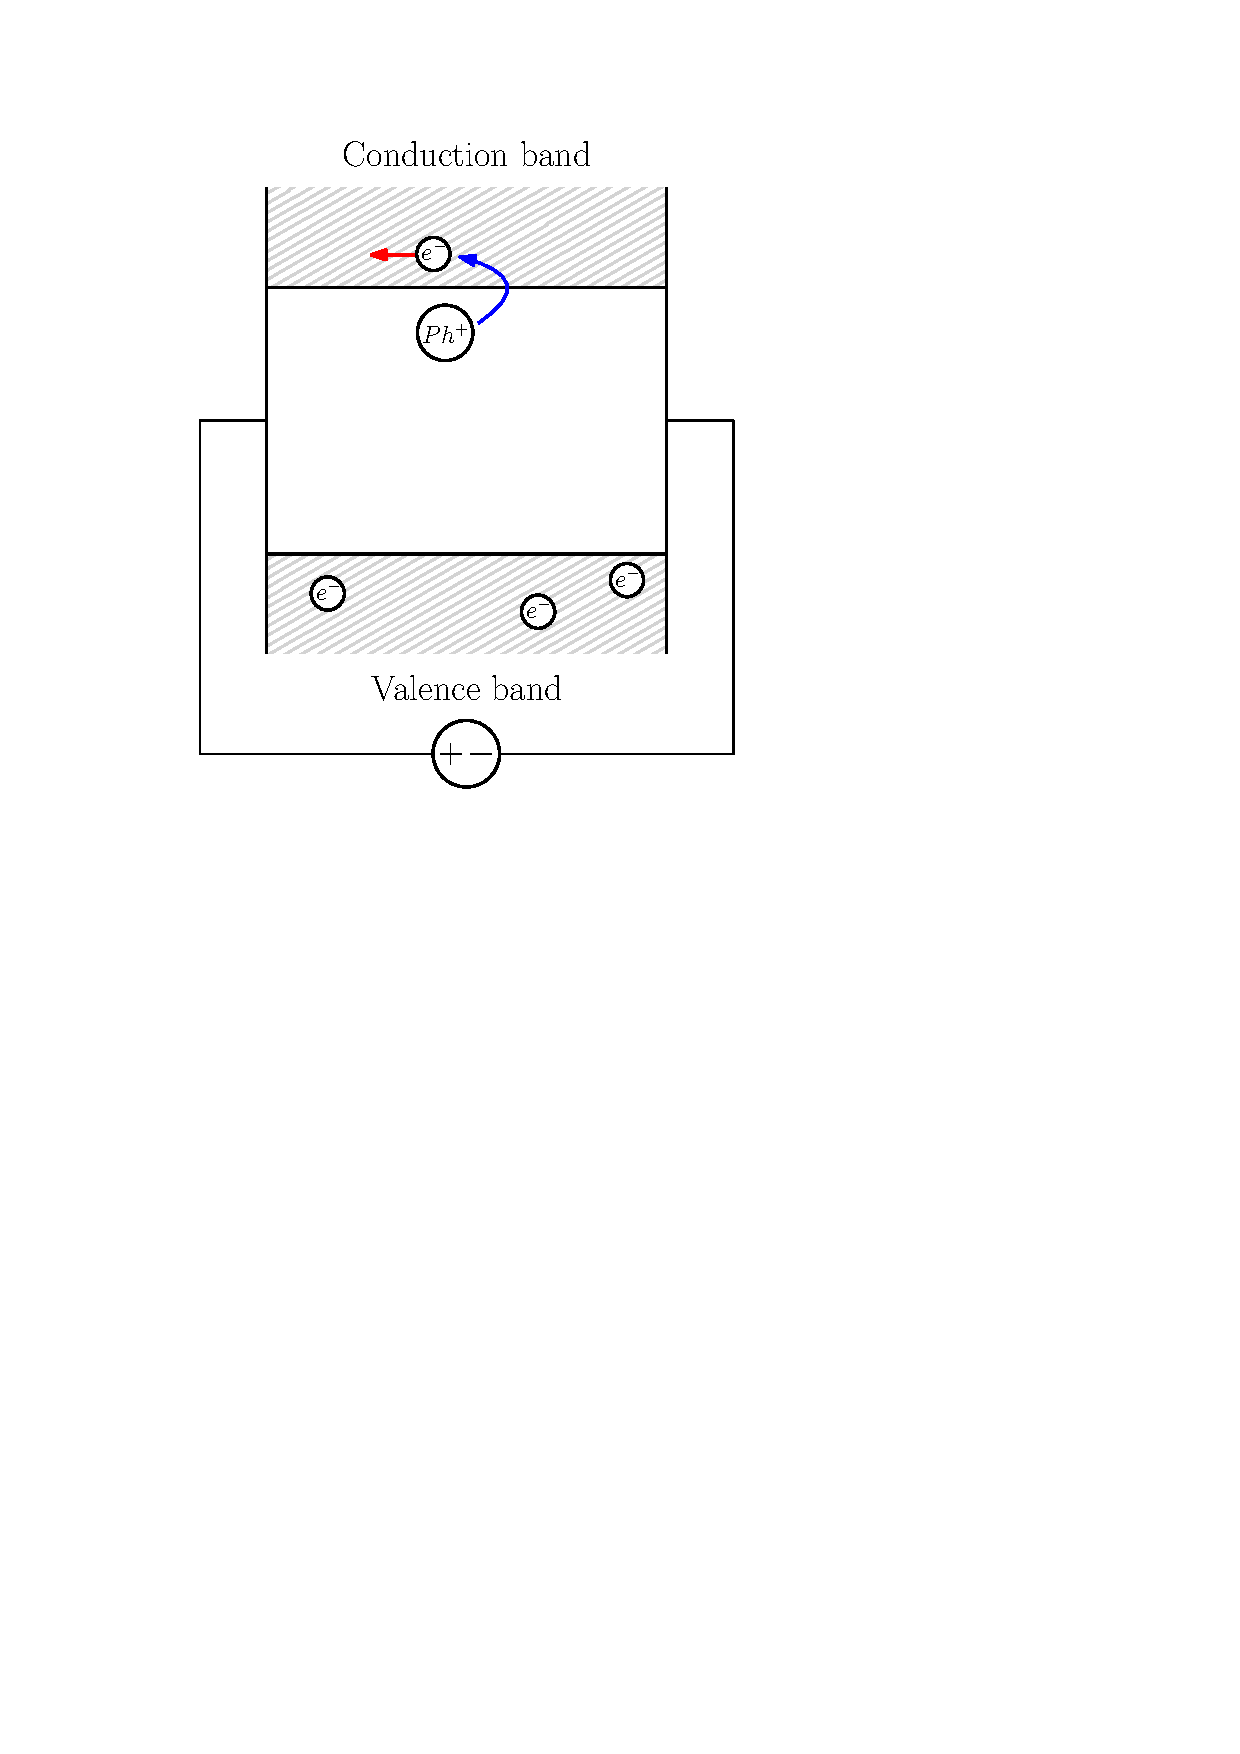
\includegraphics[scale=0.5]{n_type_doping.pdf}
\caption{N-type doping.}
\end{subfigure}%
\begin{subfigure}{.5\textwidth}
\centering
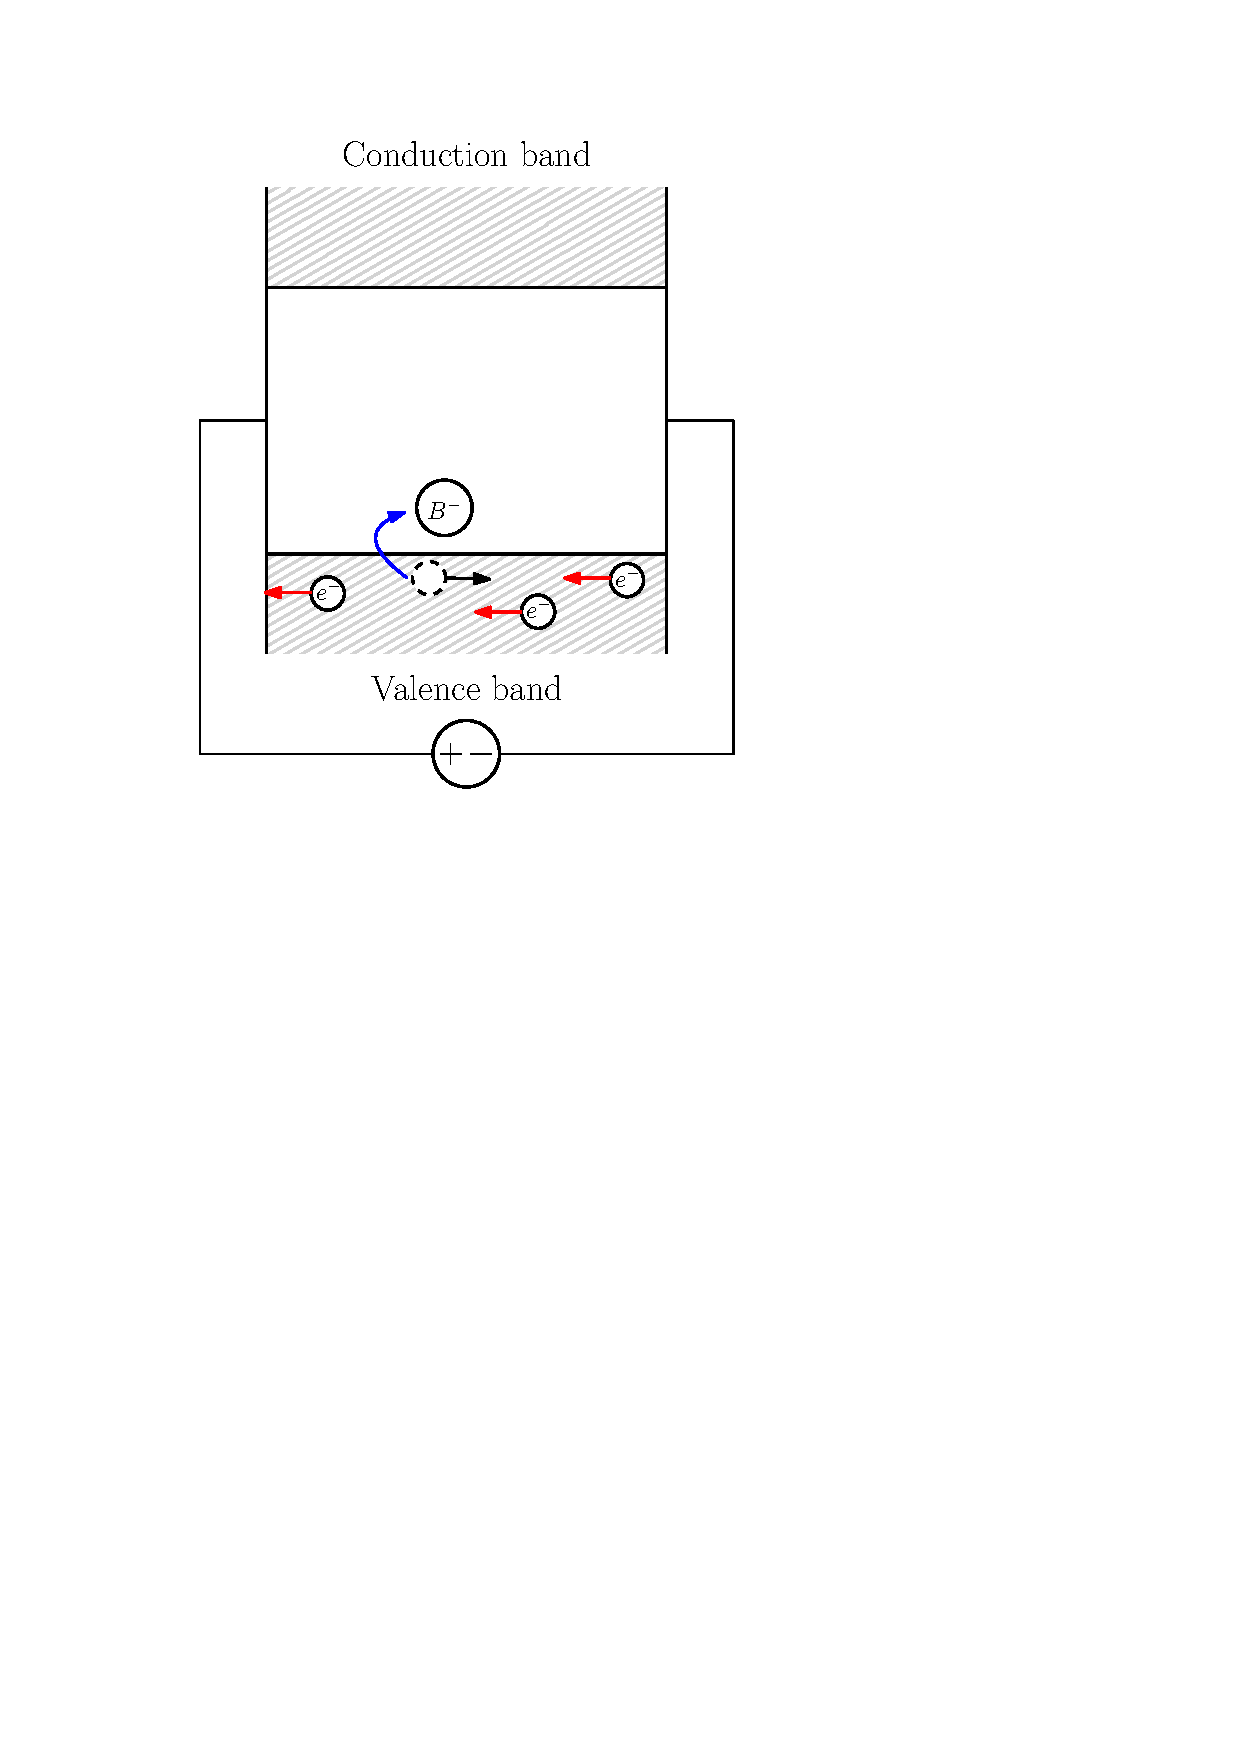
\includegraphics[scale=0.5]{p_type_doping.pdf}
\caption{P-type doping.}
\end{subfigure}
\end{figure}

\section{The P-N Junction}
On their own, doped semiconductors don't seem very interesting. However, this changes when we put them together. Consider a component (known as a \emph{p-n junction}) formed by placing a p-type doped silicon crystal (known as the \emph{P-side}) adjacent to an n-type doped crystal (known as the \emph{N-side}), as shown:
\begin{center}
    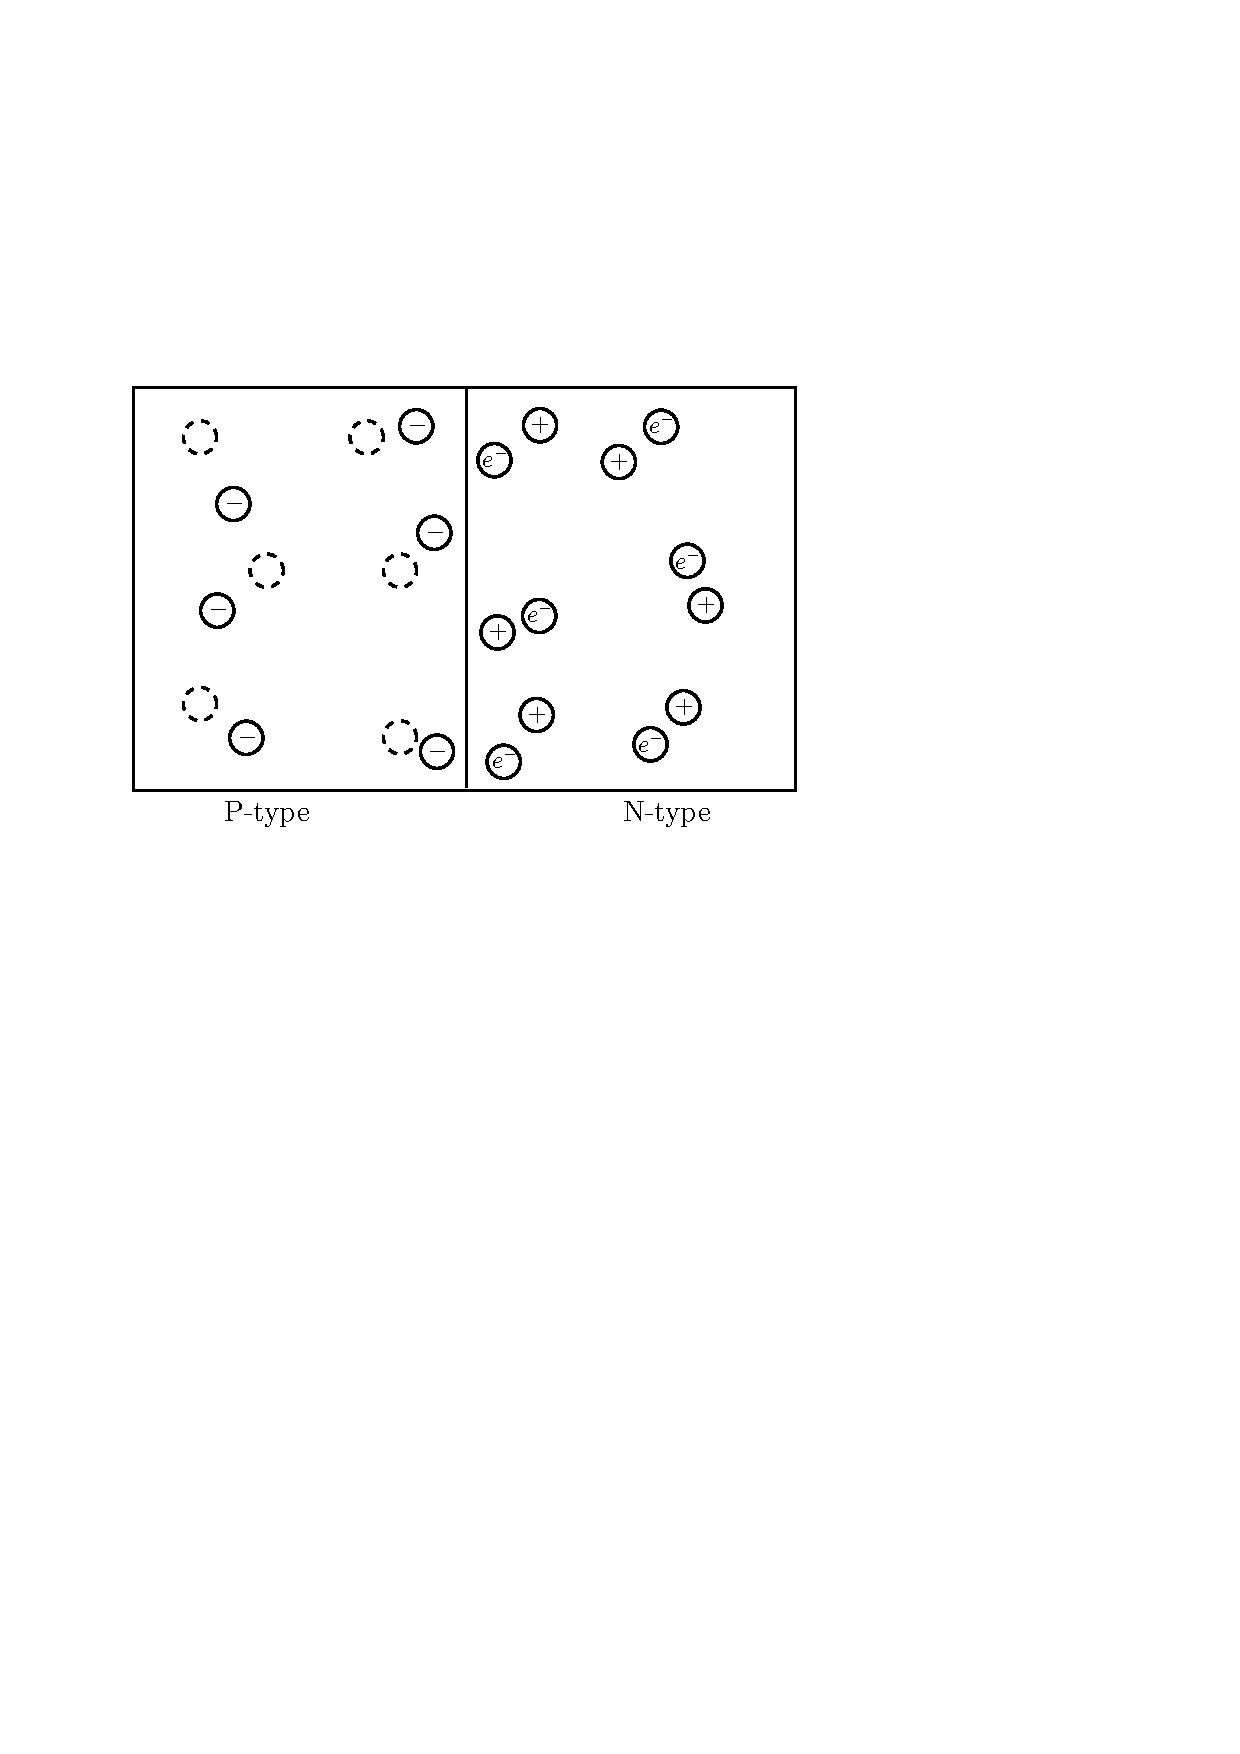
\includegraphics[scale=0.7]{p_n_junction_1.pdf}
\end{center}

Note that we are no longer drawing the energy bands explicitly, but are instead simply showing the charge carriers - positively charged holes in the P-side, and negatively charged electrons in the N-side. Note that the ions in both regions are static, and so are not charge carriers. As it turns out, at the junction of these regions (known as the \emph{depletion region}), there is a sort of ``diffusion" of charge carriers, where some positively charged holes drift over to merge with negatively charged electrons, and vice versa. Thus, at the center of this junction, no charge carriers will be present, as shown:
\begin{center}
    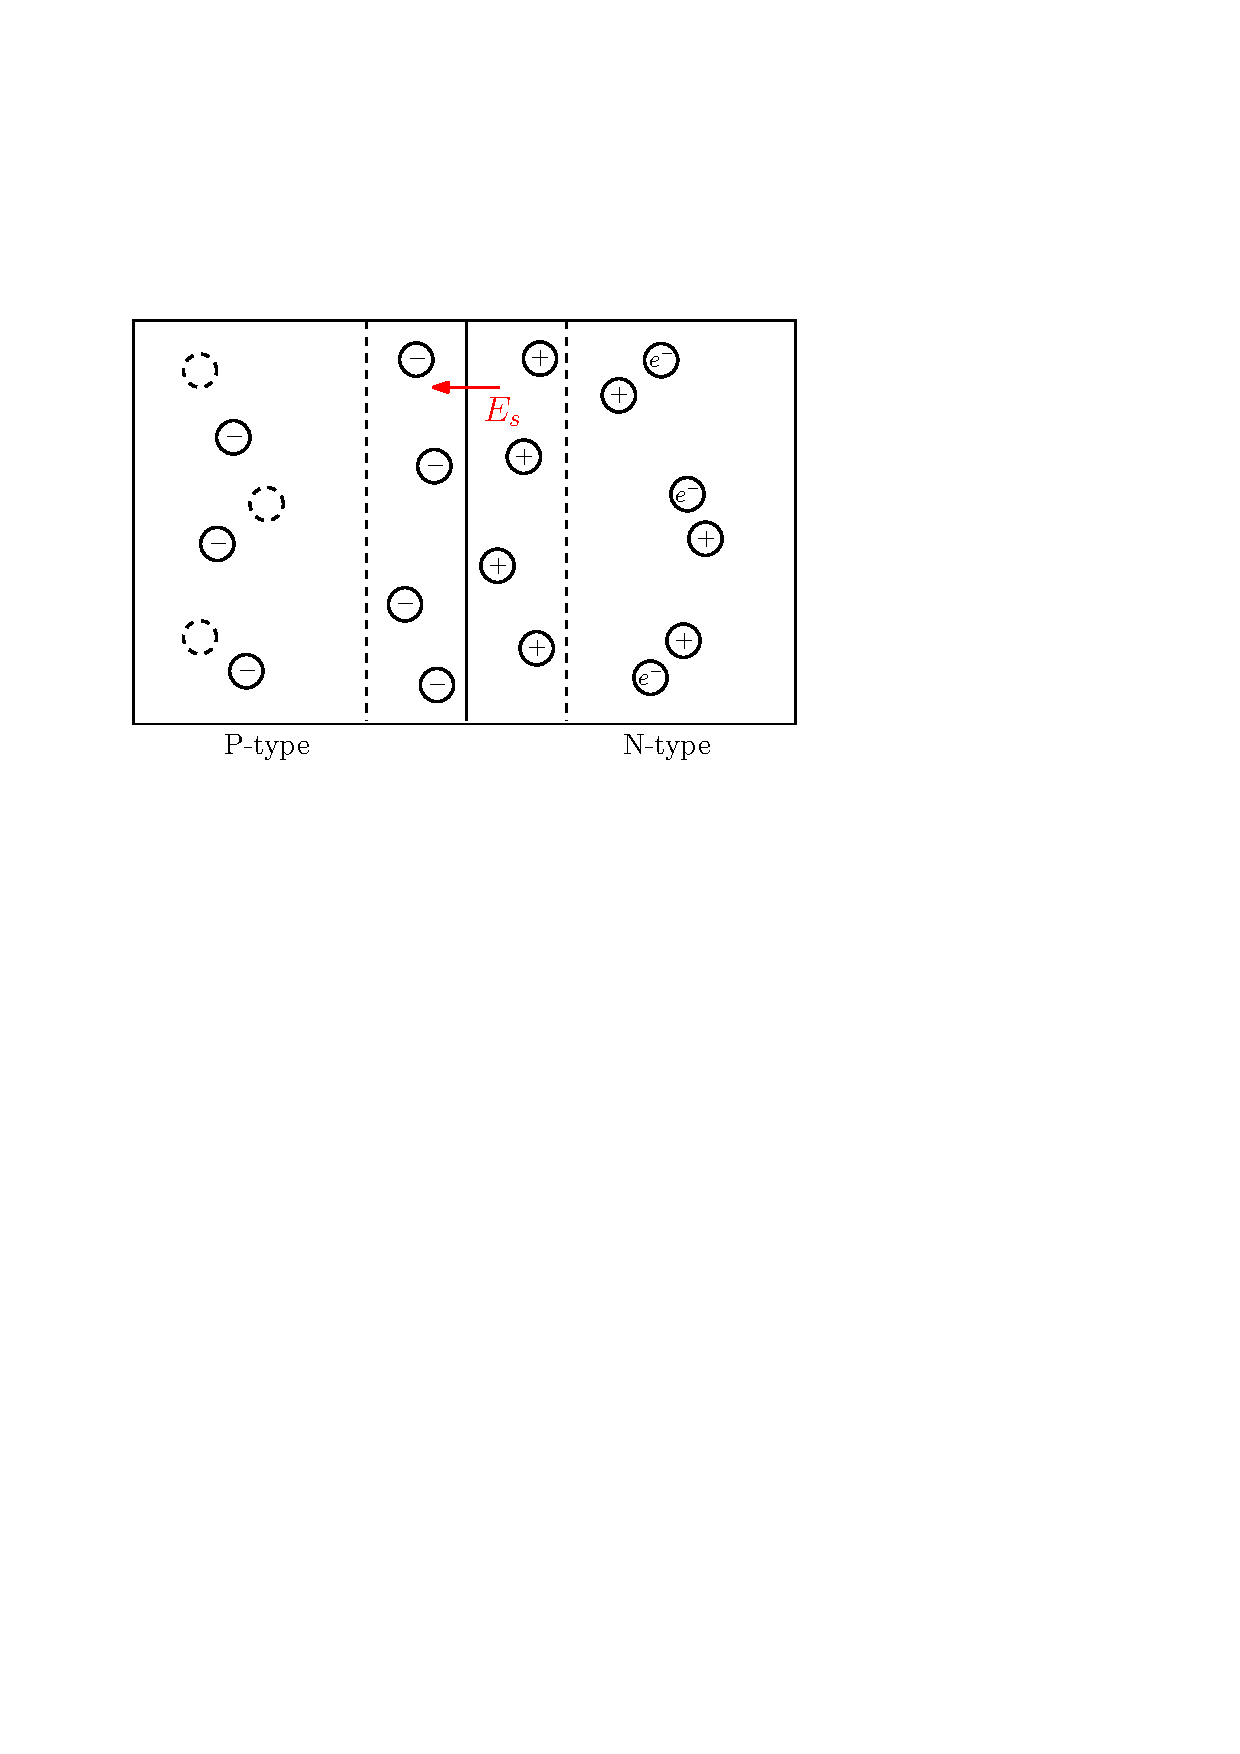
\includegraphics[scale=0.7]{p_n_junction_2.pdf}
\end{center}

A good question to ask at this point is the following: why don't \emph{all} of the charge carriers cross over and merge, leaving just the static ions? To resolve this, notice that at the middle of the interface, there are a large number of negative charges to the left and positive charges to the right, producing the electric field $E_s$ to the left. Thus, positively charged holes moving into this region will be pushed back to the P-side, and negatively charged electrons will be pushed back into the N-side.

\section{Diodes}
Now, consider what happens when we apply a voltage $V$ across this junction, as shown:
\begin{center}
    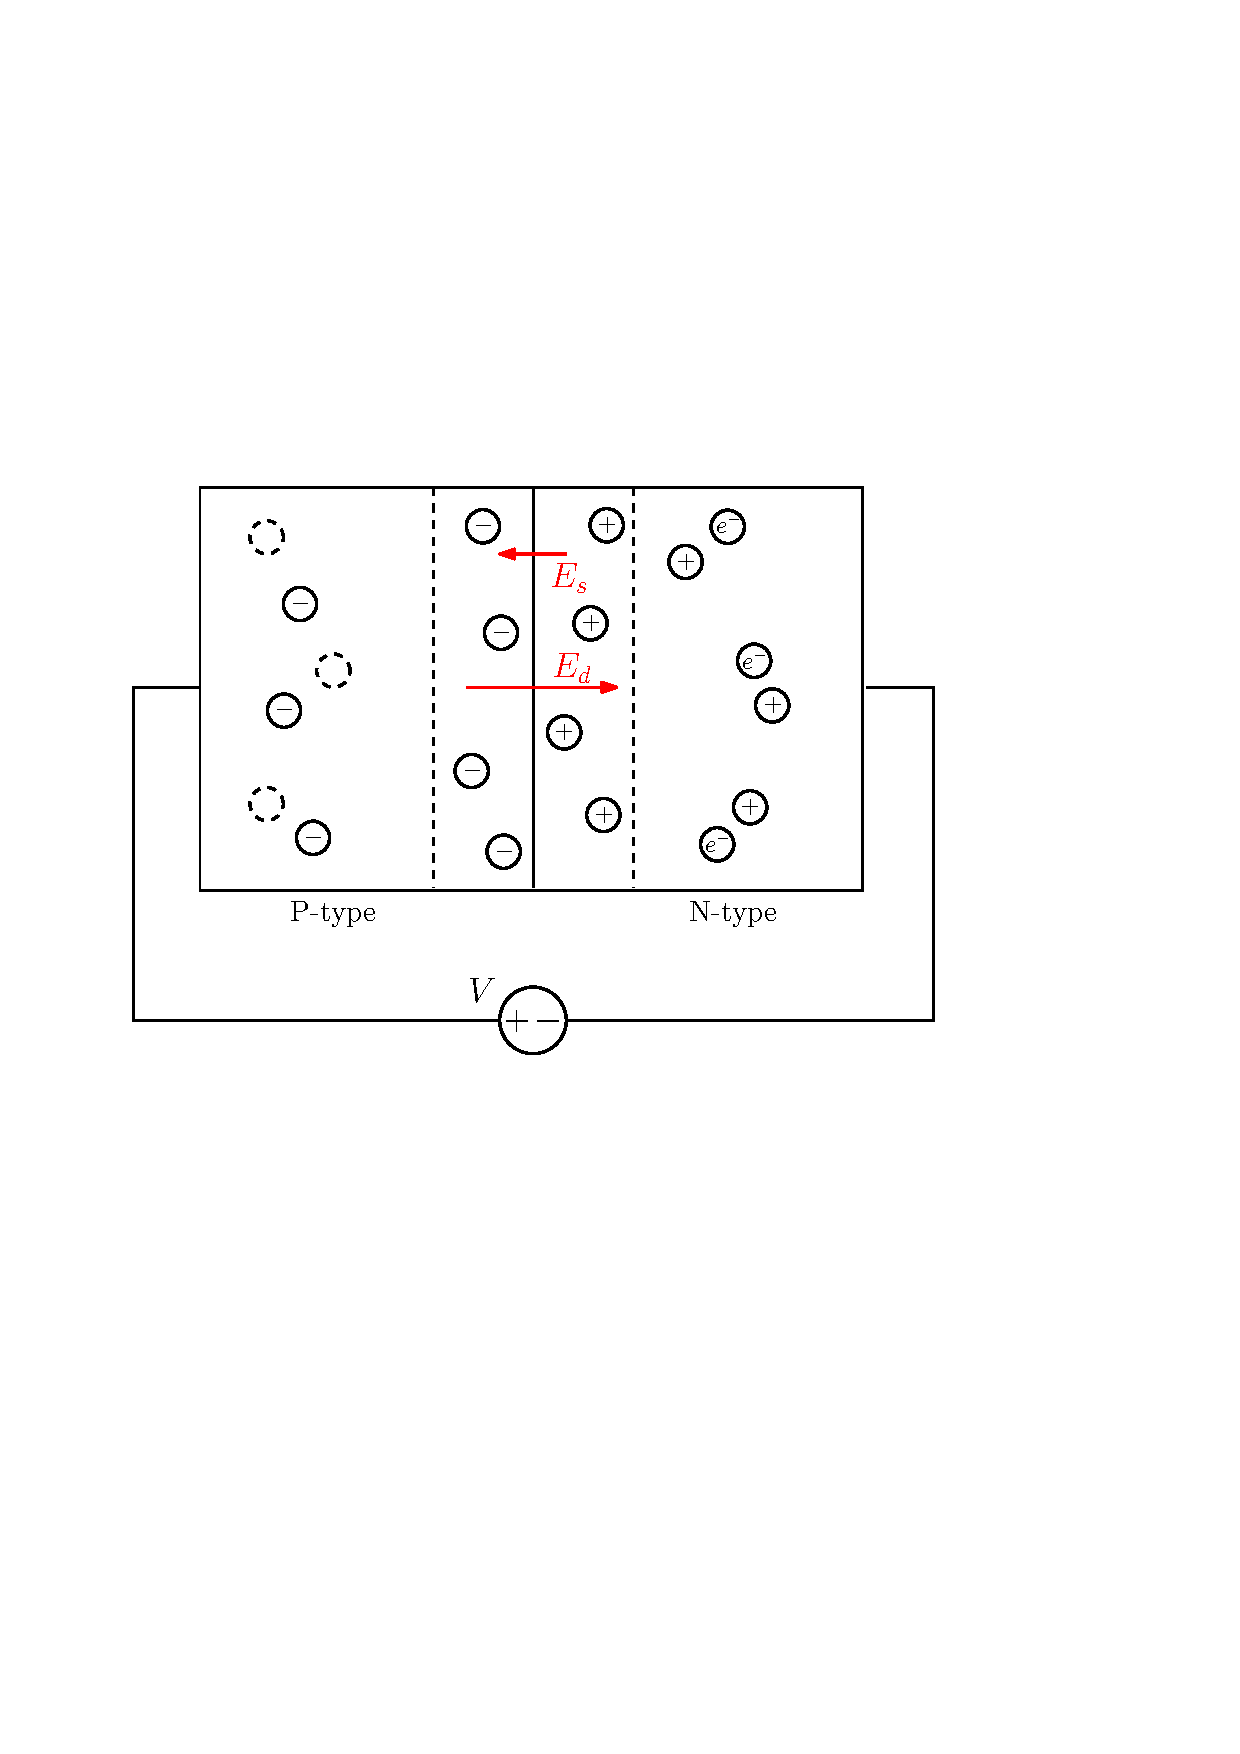
\includegraphics[scale=0.7]{p_n_junction_3.pdf}
\end{center}

If $V_d < 0$ (so the electric field driven by the voltage $E_d$ within the semiconductor goes from from right to left), we simply strengthen the electric field (since $E_s$ and $E_d$ point in the same direction) near the middle of the interface, making it even less likely for charges to flow across the barrier. However, if $V_d > 0$, then we weaken the electric field at the center of the interface (as $E_d$ opposes $E_s$), allowing charges to rush across the junction, inducing a large current. Thus, we see that this component effectively allows current to flow in one direction - in other words, it is a \emph{diode}.

The above analysis is a simplified form of the ideal behavior of a p-n junction diode. We will now present, without proof, the I-V relation for this diode:
\[
    I_D = I_S(e^{V_D / V_{th}} - 1).
\]
Here, $I_D$ is the diode current, $V_D$ is the voltage applied across the diode (as shown above), $I_S$ is a constant of the material geometry, and $V_{th}$ is the \emph{thermal voltage} of the junction. It is the case that 
\[
    V_{th} = \frac{k_BT}{e},
\]
where $T$ is the ambient temperature, and $k_B$ is the Boltzmann constant. Notice that for values of $V_D < 0$, $I_D$ can be negative, approaching $I_S$ for very large negative values of $V_D$. The mechanism for this effect is out of scope.

However, it turns out that this equation behaves very similarly to our previous model. Substituting in known values for $e$ and $k_B$, and letting the diode be at room temperature $T = \SI{300}{\kelvin}$, we find that
\[
    V_{th} \approx \SI{25.85}{\milli\volt},
\]
which is an extremely small value.

For typical material geometries, we find that $I_S$ is of the order of $10^{-12}$ amperes. Thus, it may appear, since $I_D \propto I_S$, that $I_D$ will also be very small. However, this fails to take into account the exponential term in the coefficient of $I_S$. For $V_D = \SI{1}{\volt}$, a reasonably voltage, we find that
\eqn{
    && I_D &= I_S(e^{V_D / V_{th}} - 1) \\
    &&&\approx I_S(e^{38.68} - 1) \\
    &&&\approx I_S(6.28 \times 10^{16} - 1) \\
    &&&\approx I_S(6.28 \times 10^{16}) \\
    &&&\approx \SI{62800}{\ampere},
}
which is an extremely large current for most lab applications. Thus, due to the small magnitude of $V_{th}$ and the exponential dependence in the equation for $I_D$, we are able to offset the effects of the small value of $I_S$.

We will now consider the case where $I_D = \SI{1}{\ampere}$. Solving for $V_D$,
\eqn{
    && I_D &= I_S(e^{V_D / V_{th}} - 1) \\
    \thus e^{V_D / V_{th}} &= \frac{I_D}{I_S} + 1 \\
    \thus V_d &= V_{th} \ln{\frac{I_D}{I_S} + 1} \\
    &&&\approx V_{th} \ln{\frac{I_D}{I_S}} \\
    &&&\approx \SI{0.714}{\volt}.
}
Notice that a small increase in $V_{D}$, from just above \SI{0.7}{\volt} to \SI{1}{\volt}, gives rise to an over 10000-fold increase in current. Plotting $I_D$ against $V_D$, we obtain:
\begin{center}
\begin{tikzpicture}
\begin{axis}[
    xmin=0, xmax=1,
    ymin=-0.1, ymax=0.5,
    xlabel=$V_D$ (V), ylabel=$I_D$ (A),
]
\addplot [mark=none, dashed] coordinates {(0.65, -1) (0.65, 1)};
\addplot [domain=0:0.7, samples=100] {10^(-12) * e^(x / (25.85 / 1000))};
\end{axis}
\end{tikzpicture}
\end{center}

We see that the current appears to rapidly increase for $V_D > \SI{0.65}{\volt}$. This threshold is known as the \emph{knee voltage}, and is between \SI{0.6}{\volt} and \SI{0.7}{\volt} for silicon diodes. Note that changing the scale of the graph will affect the position of the knee voltage, but the values seen here are valid for typical scale levels.

\section{Solar Cells and Photodiodes}
Recall that electrons within a semiconductor are excited by the impact of a photon. We will now use this property in order to create a solar cell, which generates power when exposed to light. Consider the impact of a photon in the depletion region of a p-n junction, as shown:
\begin{center}
    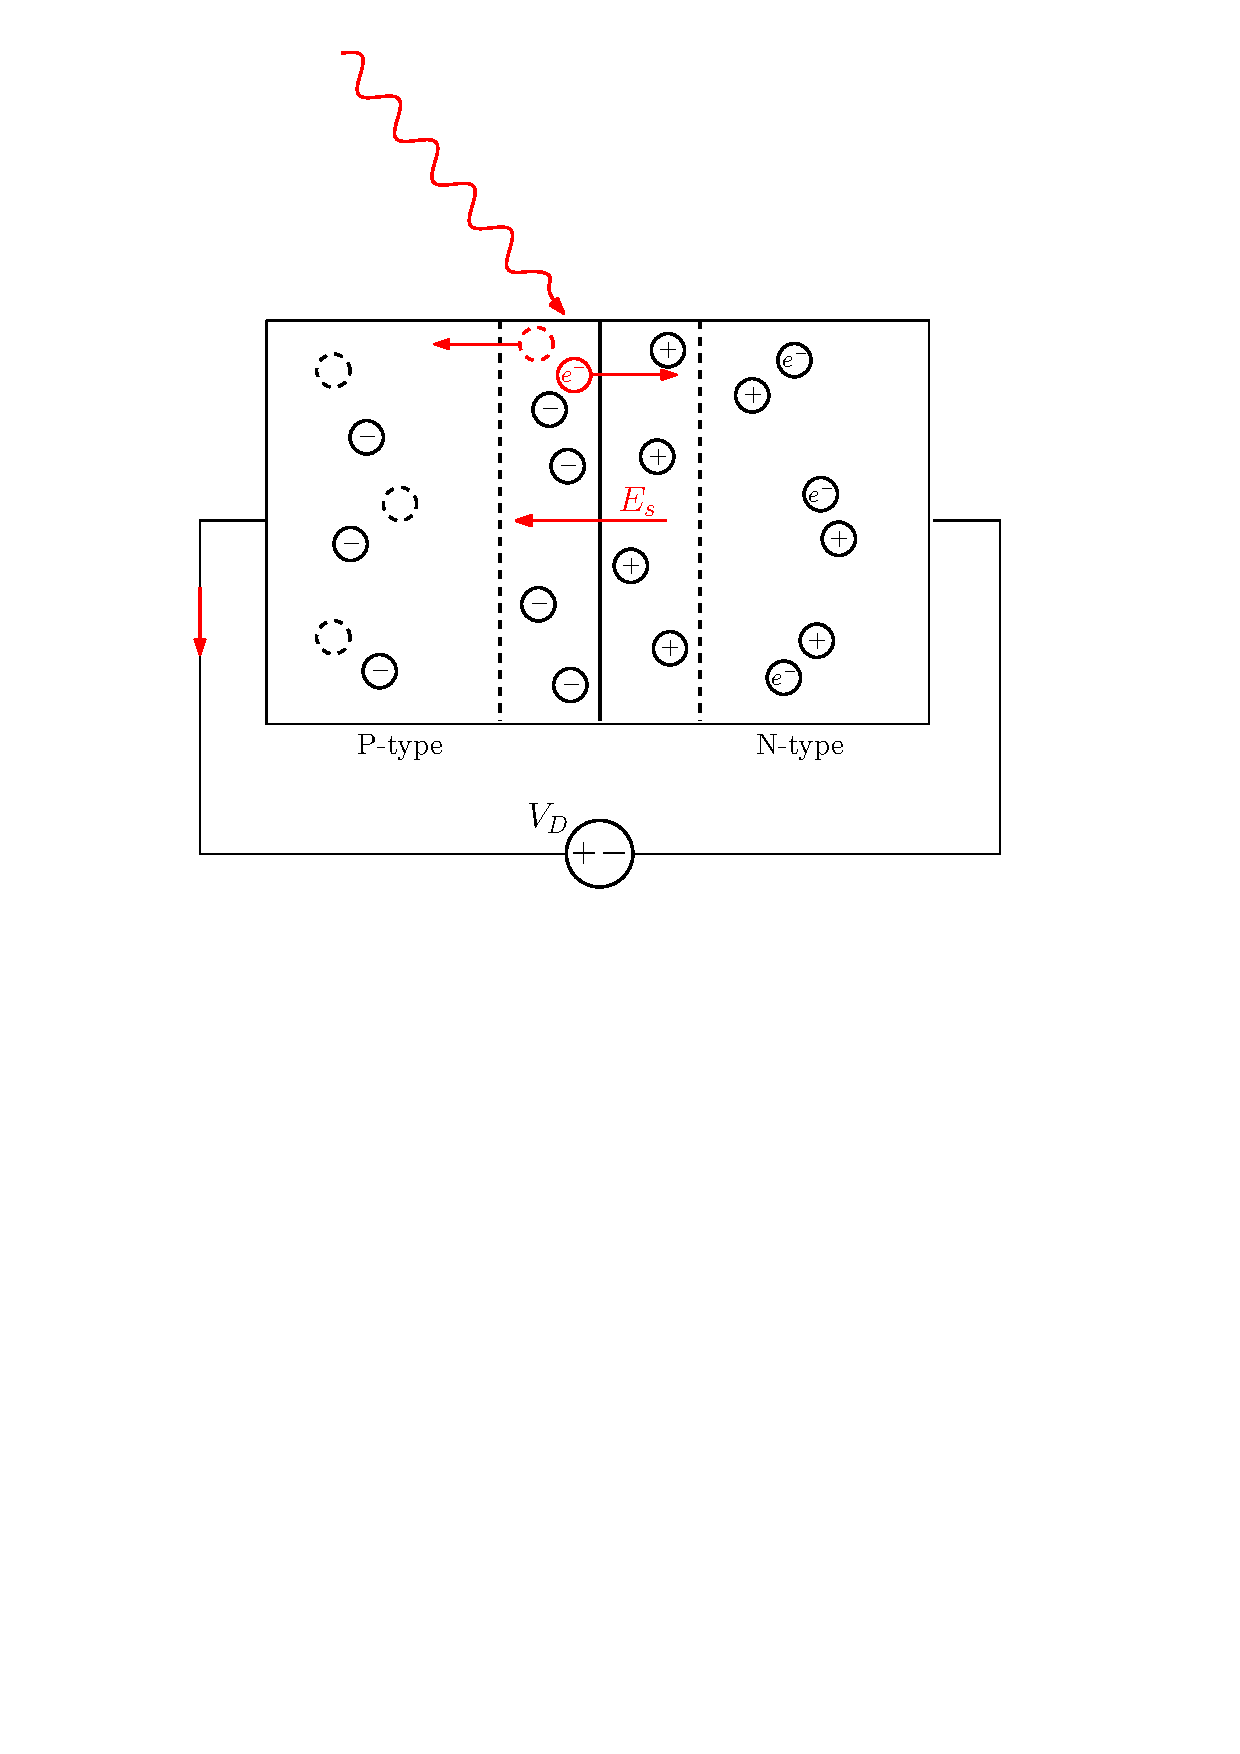
\includegraphics[scale=0.7]{photodiode.pdf}
\end{center}

When the photon impacts, it excites an electron, producing a hole and an electron. The electric field $E_s$ pulls the electron into the N-side and the hole into the P-side. This induces a current against the voltage supply, which generates energy (since this current goes against the voltage supply, we term it \emph{negative current}). Note that in the absence of light, the voltage supply drives a positive current through the junction, wasting energy.

When attempting to measure levels of light precisely, this positive current is undesirable. To eliminate it almost entirely, we can reverse the direction of the voltage supply, setting $V < 0$. Here, in the absence of light, no current will flow. However, when a photon impacts the depletion region, it will drive current through the power supply, but this time the current will be from a high voltage to a low one (since $0 > V$). Thus, negative values of $V_D$ cause energy to be consumed, not generated, in the presence of light - in this case, the component is called a \emph{photodiode}, not a solar cell.

The following plot illustrates the movement of the I-V curve of a solar cell in the presence of light:
\begin{center}
\begin{tikzpicture}
\begin{axis}[
    xmin=0, xmax=0.8,
    ymin=-1, ymax=0.5,
    xlabel=$V_D$ (V), ylabel=$I_D$ (A),
    legend style={at={(0.03,0.97)},anchor=north west}
]
\addplot [domain=0:0.7, samples=100, dashed] {10^(-12) * e^(x / (25.85 / 1000))};
\addplot [domain=0:0.8, samples=100] {10^(-12) * e^(x / (25.85 / 1000)) - 0.5};
\addlegendentry{$I_{dark}$}
\addlegendentry{$I_{light}$}
\end{axis}
\end{tikzpicture}
\end{center}
Notice that $I_{light}$ is negative, since the current moves against $V_D$. To maximize the power generated by a solar cell, we must select a $V_D$ that maximizes the product $P = -I_DV_D$, which lies somewhere on the curve $I_{light}$.

\section{LEDs}
Observe that when we drive current forward through a p-n junction, we waste energy. The energy is dissipated when an electron joins with a positive hole, as the electron must then drop from the conduction energy band down to the valence energy band. Normally, this energy is dissipated as heat. However, it is possible to construct diodes where this energy is instead radiated outwards as a photon, whose energy corresponds to the band gap between the energy bands. Such a light emitting diode is known as a \emph{light emitting diode}\footnote{super original, right?}, or LED. By constructing our LED carefully, we can reduce the energy dissipated as heat to almost $0$, making LEDs extremely efficient light sources.

One property of LEDs is that they emit functionally monochromatic light (light of approximately a single frequency), since the frequency of their emitted light depends solely on the band gap of the diode, which is a constant. To change the color of the light, we must use different semiconducting materials - for instance, to produce green light, we must make our LED out of a gallium nitride crystal. As it turns out, we cannot make LEDs out of silicon, since the photon whose energy corresponds to the band gap of silicon lies in the infrared spectrum, not the visible spectrum.

\section{Bipolar Junction Transistors}
Finally, we will discuss how semiconductors enable the creation of transistors. Consider the following configuration of N-type and P-type doped regions:
\begin{center}
    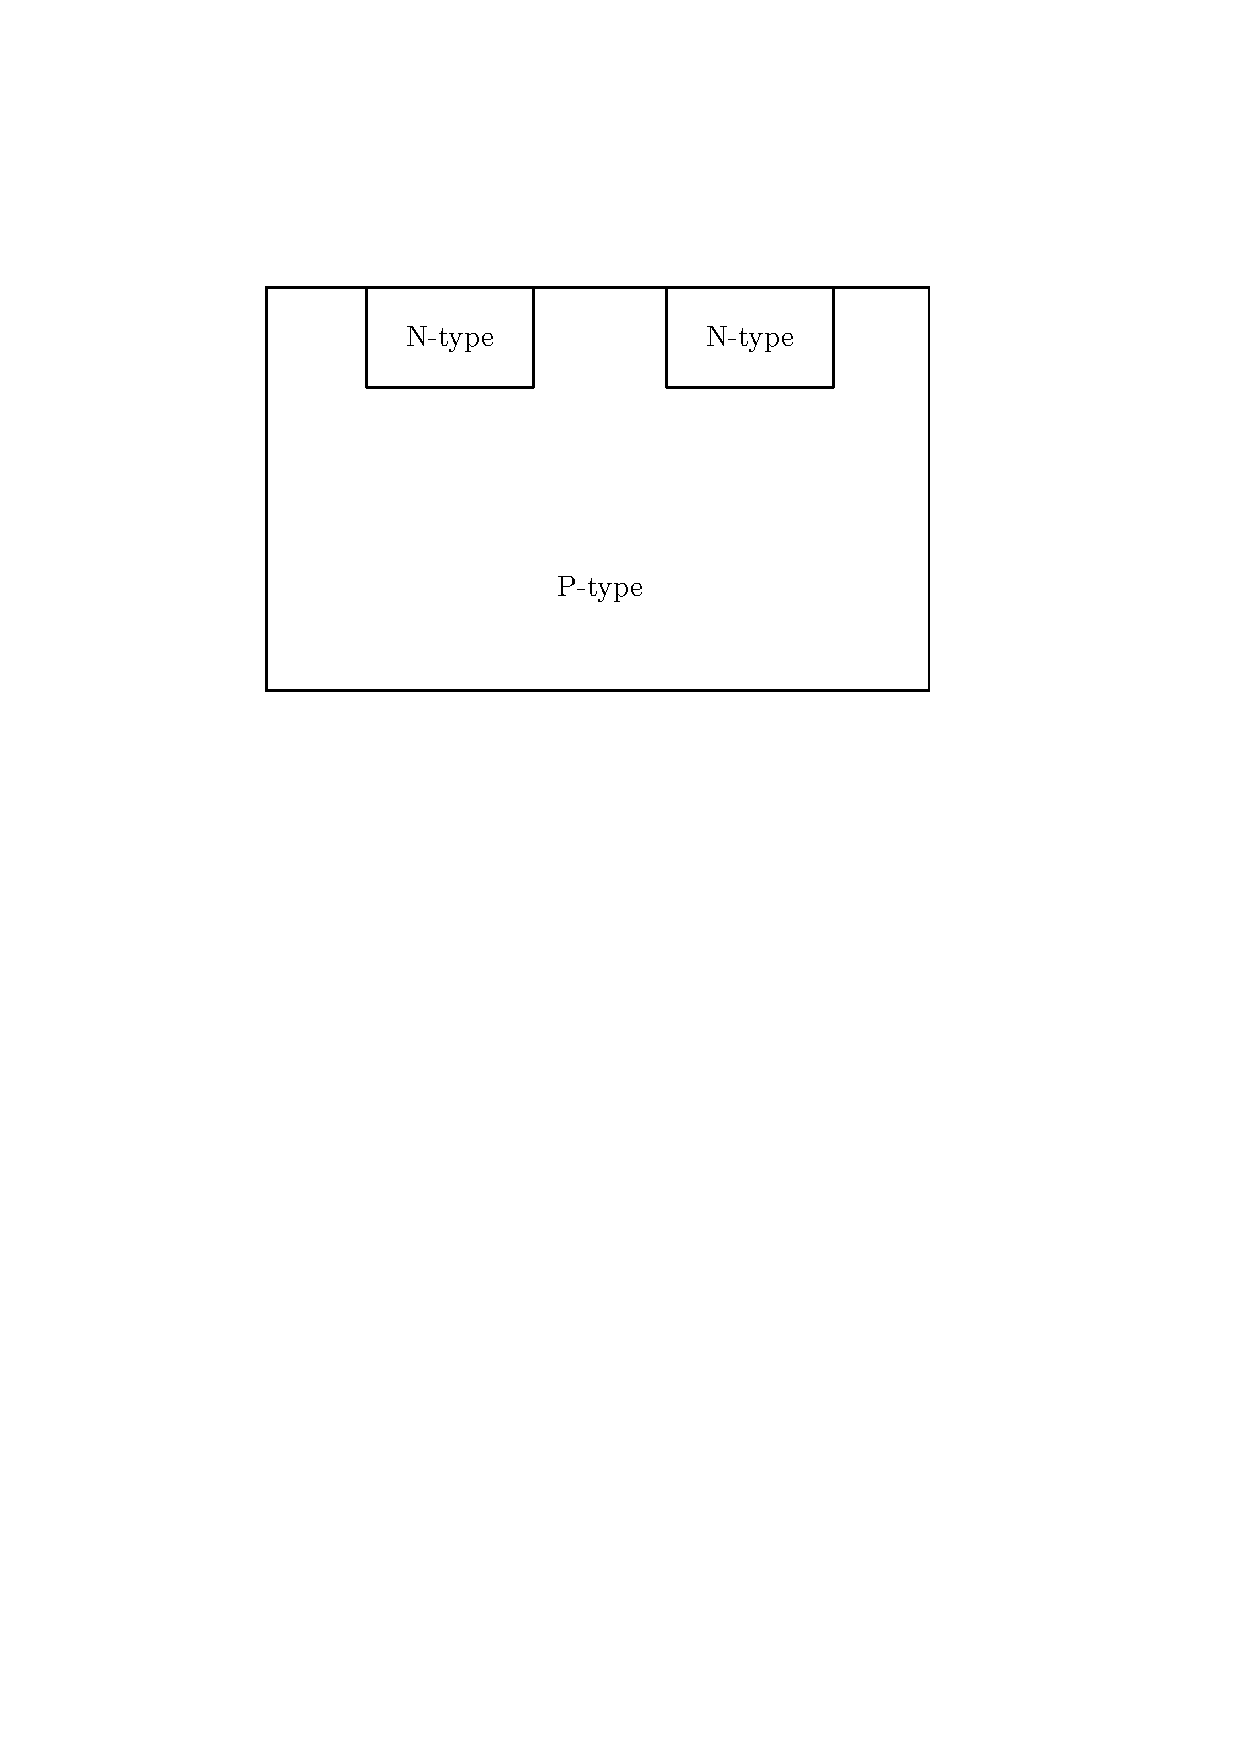
\includegraphics[scale=0.7]{bipolar_transistor.pdf}
\end{center}

We can imagine this configuration as being two diodes connected at a common terminal, as follows:
\begin{center}
\begin{circuitikz}[american]
\draw (0, 0) node[circ]{};
\draw (0, 0) to[diode] (-2, 2) node[circ]{};
\draw (0, 0) to[diode] (2, 2) node[circ]{};
\end{circuitikz}
\end{center}

We will attach voltage sources to the three terminals of this component, as follows:
\begin{center}
\begin{circuitikz}[american]
\draw (0, 0) node[circ]{} node[below]{$V_a$};
\draw (0, 0) to[diode, i=$I_1$] (-2, 2) node[circ]{} node[left]{$V_{DD}$};
\draw (0, 0) to[diode, i=$I_2$] (2, 2) node[circ]{} node[ground]{};
\end{circuitikz}
\end{center}
We will set $V_{DD} \approx \SI{10}{\volt}$, and vary $V_a$ from \SI{0}{\volt} to about \SI{0.7}{\volt} (the knee voltage of our diodes).

Observe that as we raise $V_a$, the right diode will become forward biased and start to conduct, but the left diode will be reverse biased, so $I_1 \approx 0$. As we reach the knee voltage, $I_2$ will rise to a relatively large value. Recall from our understanding of p-n junctions that, in diodes conducting current, electrons will flow out of the N-type region, into the P-type region. However, if the two N-type regions are placed together in a suitable manner, most of these electrons will encounter the other N-type region, and be pulled by $V_{DD}$ through the diode. Thus, the left diode will become conducting as well. This mechanism is summarized in the below figure:
\begin{center}
    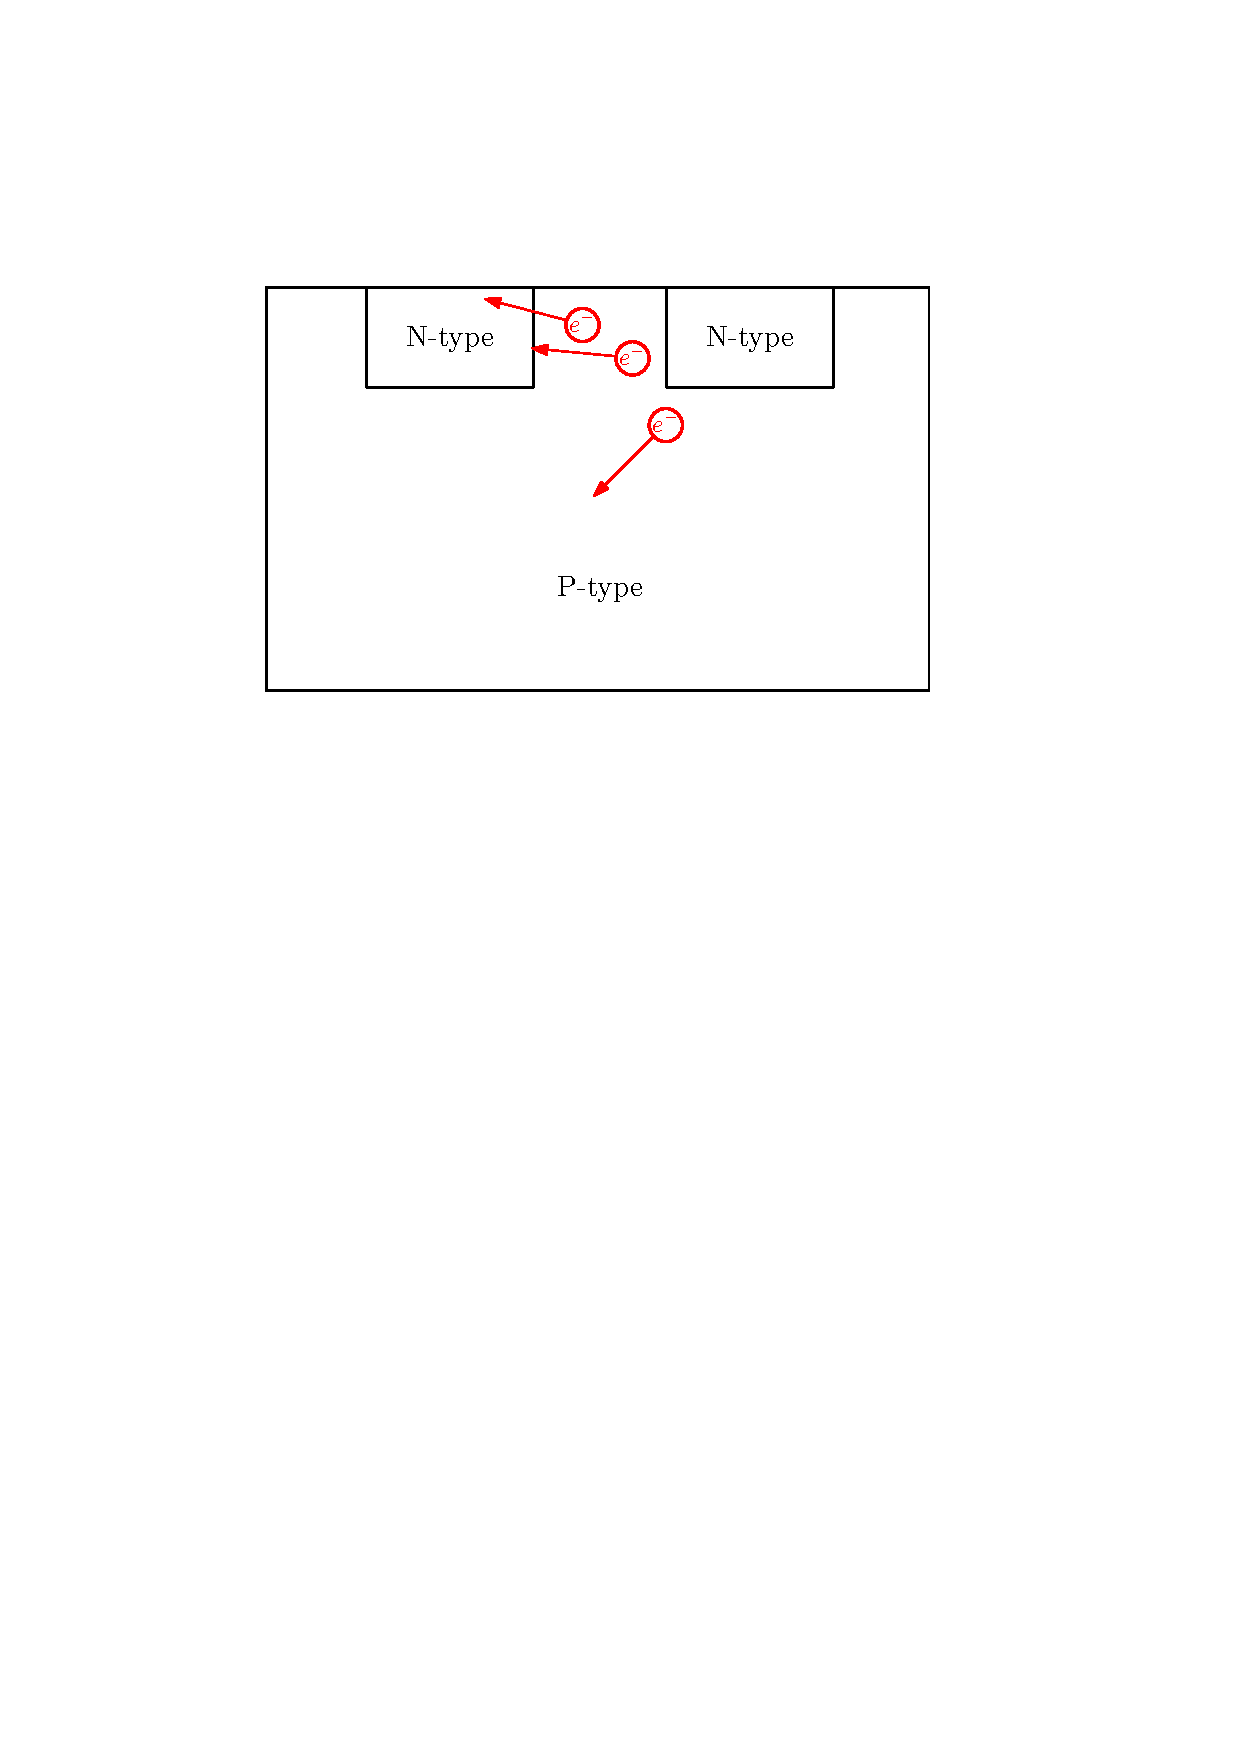
\includegraphics[scale=0.7]{bipolar_transistor_conducting.pdf}
\end{center}
We call the rightmost N-type doped region the \emph{emitter}, and the leftmost N-type doped region the \emph{collector}, due to this motion of electrons. We call the point where the P-type region is connected to $V_a$ the \emph{base}. Thus, we see that when we raise the voltage at the base past some threshold voltage, the component begins to conduct between the collector and the emitter. Thus, this component is a transistor - known as a \emph{bipolar junction transistor}.

\section{MOSFETS}
However, one issue with the previous transistor is the fact that, for values of $V_a$ greater than zero but less than the knee voltage, current will be drawn from the base to the emitter. This is undesirable, and to address this we will construct another type of transistor, where no current is ever drawn from the control node.

We will make a small modification to our bipolar transistor, by placing a sheet of glass on the outside of the P-type region, near the two N-type regions. On top of this sheet of glass we will place a sheet of aluminium, as shown:
\begin{center}
    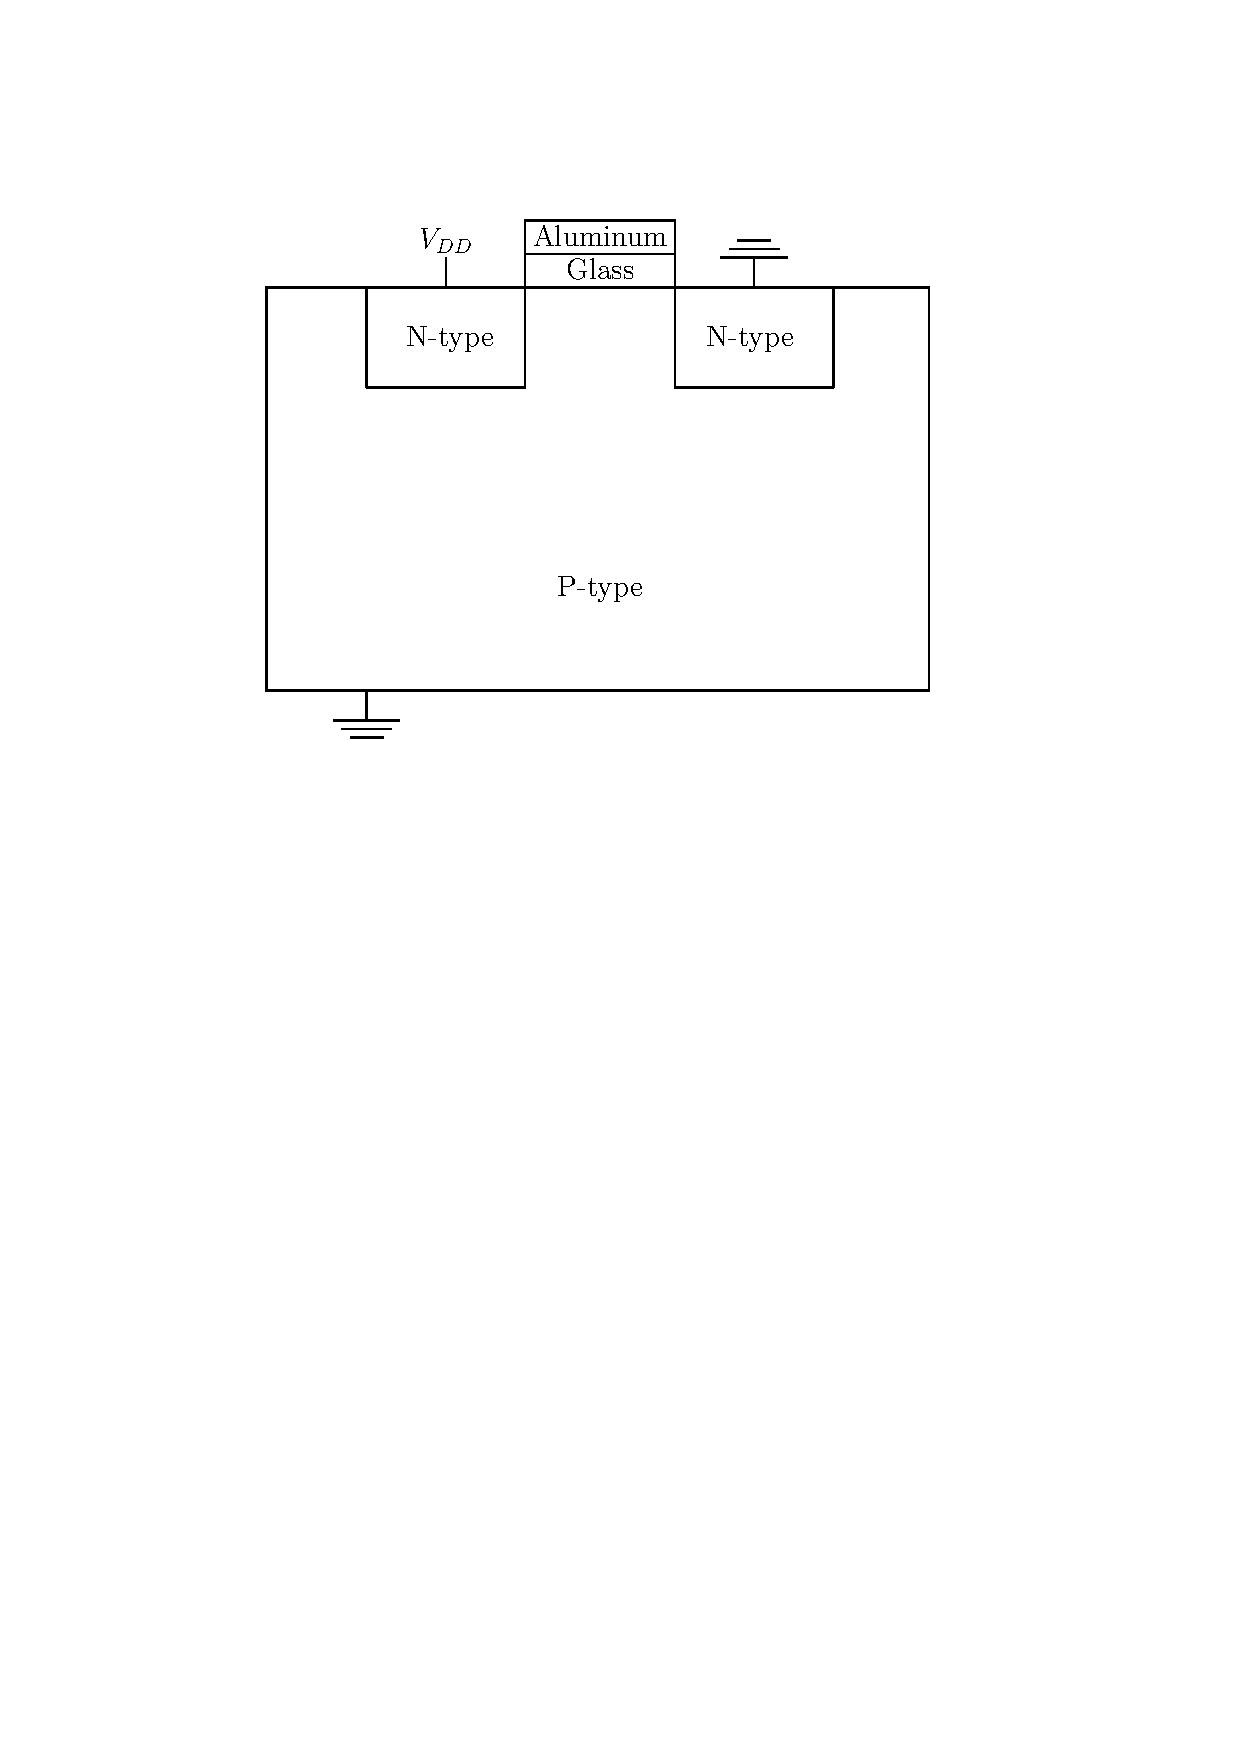
\includegraphics[scale=0.7]{mosfet.pdf}
\end{center}
We will refer to the sheet of aluminium as the \emph{gate}, and apply a positive voltage $V_a$ to it. As this voltage passes some threshold $V_{th}$, it repels positive holes in its vicinity. We assert, without proof, that the portion of the P-type region in the vicinity of the gate will begin to behave more like a N-type region, allowing electrons in the conduction bands of the adjacent true N-type regions to flow freely. Due to the voltages applied, electrons will be drawn from the rightmost N-type region by the voltage $V_{DD}$, draining into the leftmost N-type region. Thus, we will refer to the rightmost N-type region as the \emph{source}, and the leftmost N-type region as the \emph{drain}. This mechanism is summarized below:
\begin{center}
    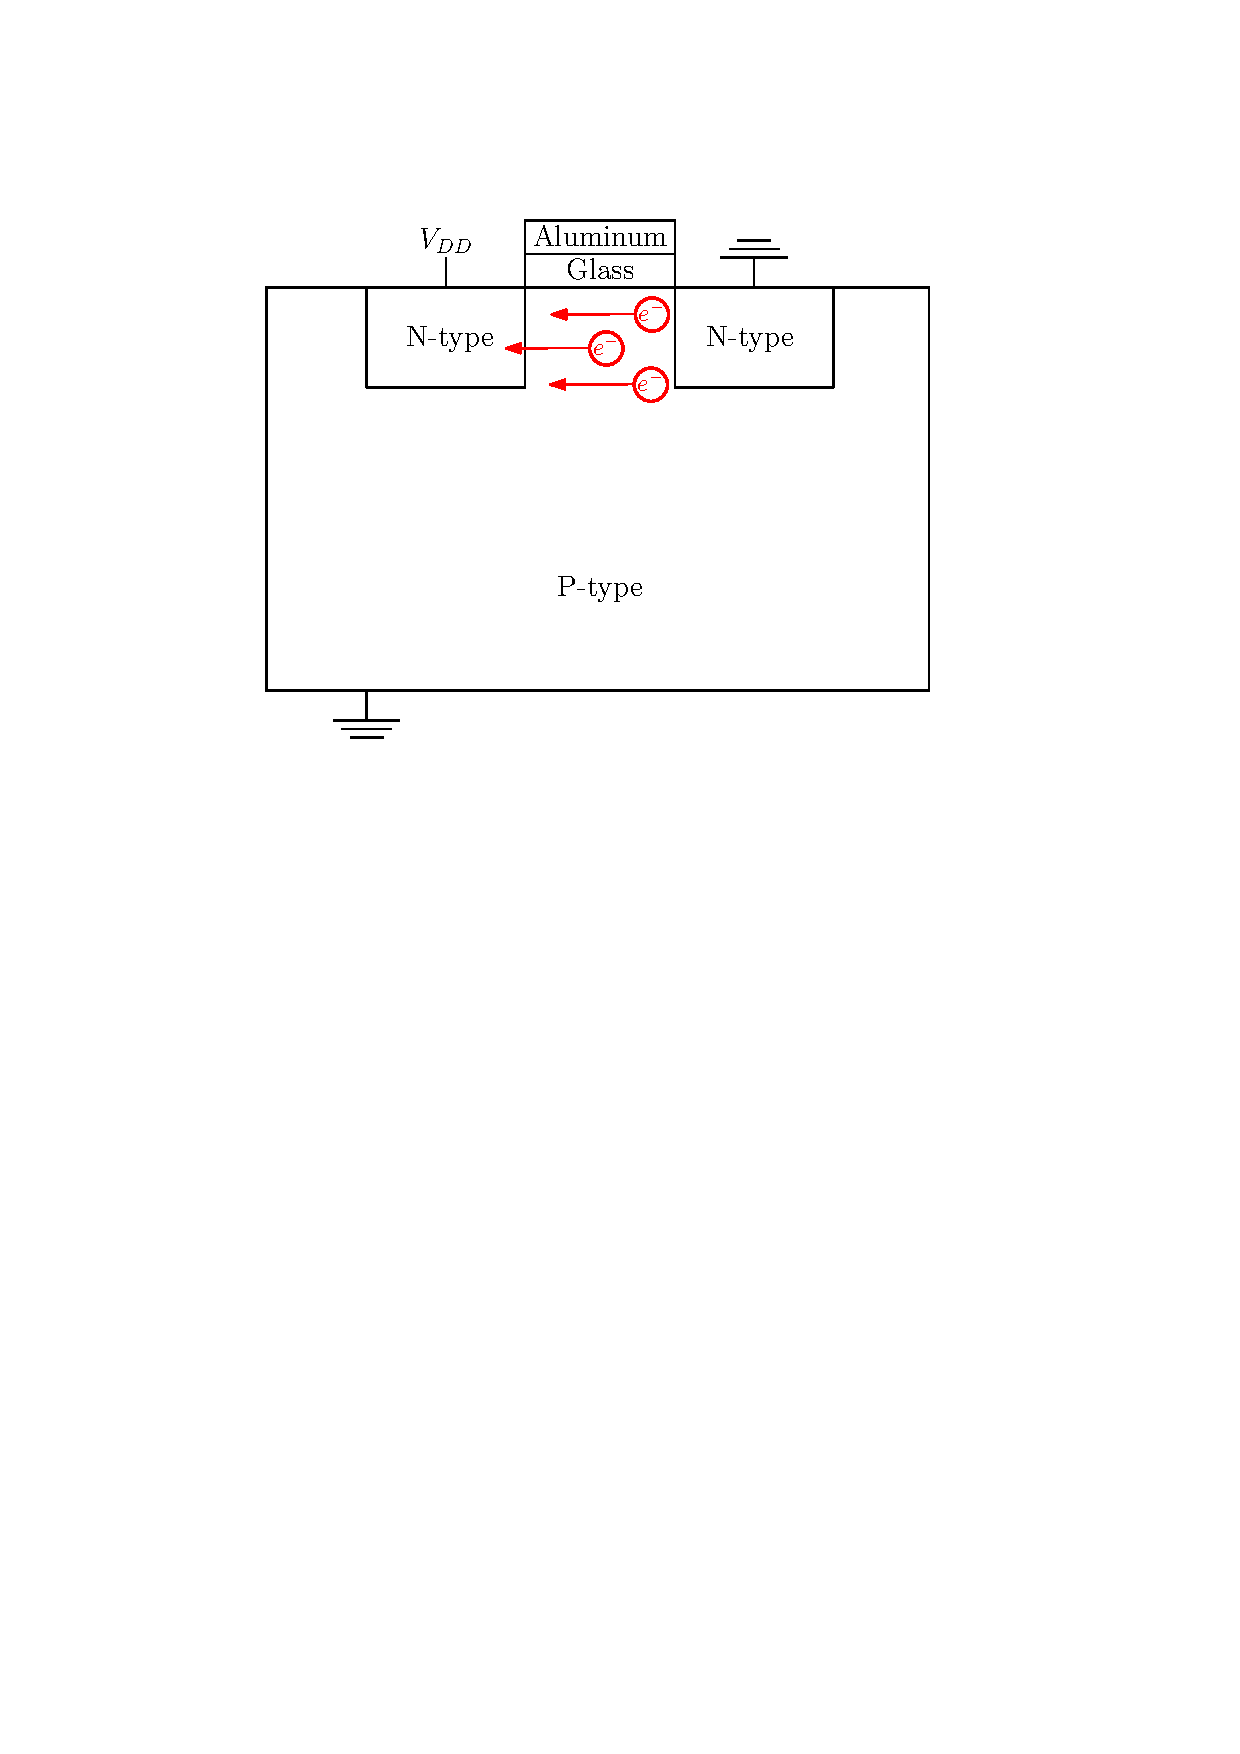
\includegraphics[scale=0.7]{mosfet_conducting.pdf}
\end{center}

This component clearly behaves like the transistors we're used to - specifically, an NMOS \emph{MOSFET}. Swapping the P-type and N-type doping will produce a PMOS MOSFET.

Observe that, as glass is an insulator, no current is being drawn from the gate. However, it has some capacitance with the P-type region, which we have previously observed and analyzed. This completes our discussion of semiconductor physics.

\end{document}
